%============================================================
% OptiKuh EDA Presentation
% Case-study style: setup + overview + numeric EDA findings
%============================================================

%==================== SLIDE 1: TITLE ====================
{
\setbeamertemplate{footline}{}
\begin{frame}[noframenumbering]

\vspace{1.9cm}

\begin{center}
    {\fontsize{25}{29}\selectfont \color{tugreen}
    Case Study II:\\[0.25cm]
    OptiKuh Dairy Cow Health Data}
\end{center}

\vspace{0.95cm}

\begin{flushleft}
{\large
Nixon M Paulson\\
Rohith B Chowdappa\\
Maria Cherian}
\end{flushleft}

\end{frame}
}

%==================== SLIDE 2 ====================
\begin{frame}{What we did}

\setbeamercolor{item}{fg=tugreen}
\begin{itemize}
    \item Performed exploratory data analysis on:
    \begin{itemize}
        \item dataset size and observation period
        \item missing values and measurement availability
        \item health-status distribution
        \item farm-level and breed-level differences
        \item diagnosis labels
        \item milk yield and metabolic-marker patterns
    \end{itemize}
\end{itemize}

\end{frame}

%==================== SLIDE 3 ====================
\begin{frame}{Dataset Overview}

\setbeamercolor{item}{fg=tugreen}
\begin{itemize}
    \item Daily records: 492,540
    \item Original variables: 49
    \item Unique animals: 1,714
    \item Anonymized farms: 12
    \item Approx. lactation episodes: 3,422
    \item Observation window: 2014-08-28 to 2017-03-23
\end{itemize}

\vspace{0.3cm}

\textbf{Note:} this is a large repeated-measurement dataset, not a simple one-row-per-animal dataset.

\end{frame}

%==================== SLIDE 4 ====================
\begin{frame}{Basic Data Quality Checks}

\setbeamercolor{item}{fg=tugreen}
\begin{itemize}
    \item Dates were parsed to check the 32-month observation window
    \item Animal, farm and lactation identifiers were checked for repeated measurements
    \item Missing values were checked column-wise and by measurement group
    \item Health status was summarized at lactation-episode level to avoid repeated counting
    \item Daily-record summaries and lactation-episode summaries were kept separate
\end{itemize}

\vspace{0.25cm}

\textbf{Main point:} the data must be handled according to animal, farm and lactation structure.

\end{frame}

%==================== SLIDE 5 ====================
\begin{frame}{Analysis 1.1}

\setbeamercolor{item}{fg=tugreen}
\begin{itemize}
    \item Observation period covers 32 months
    \item Monthly records range from 4 rows at the beginning to 25,852 rows at the peak
    \item Highest monthly coverage was in 2015-10
\end{itemize}

\vspace{0.15cm}

\begin{center}
    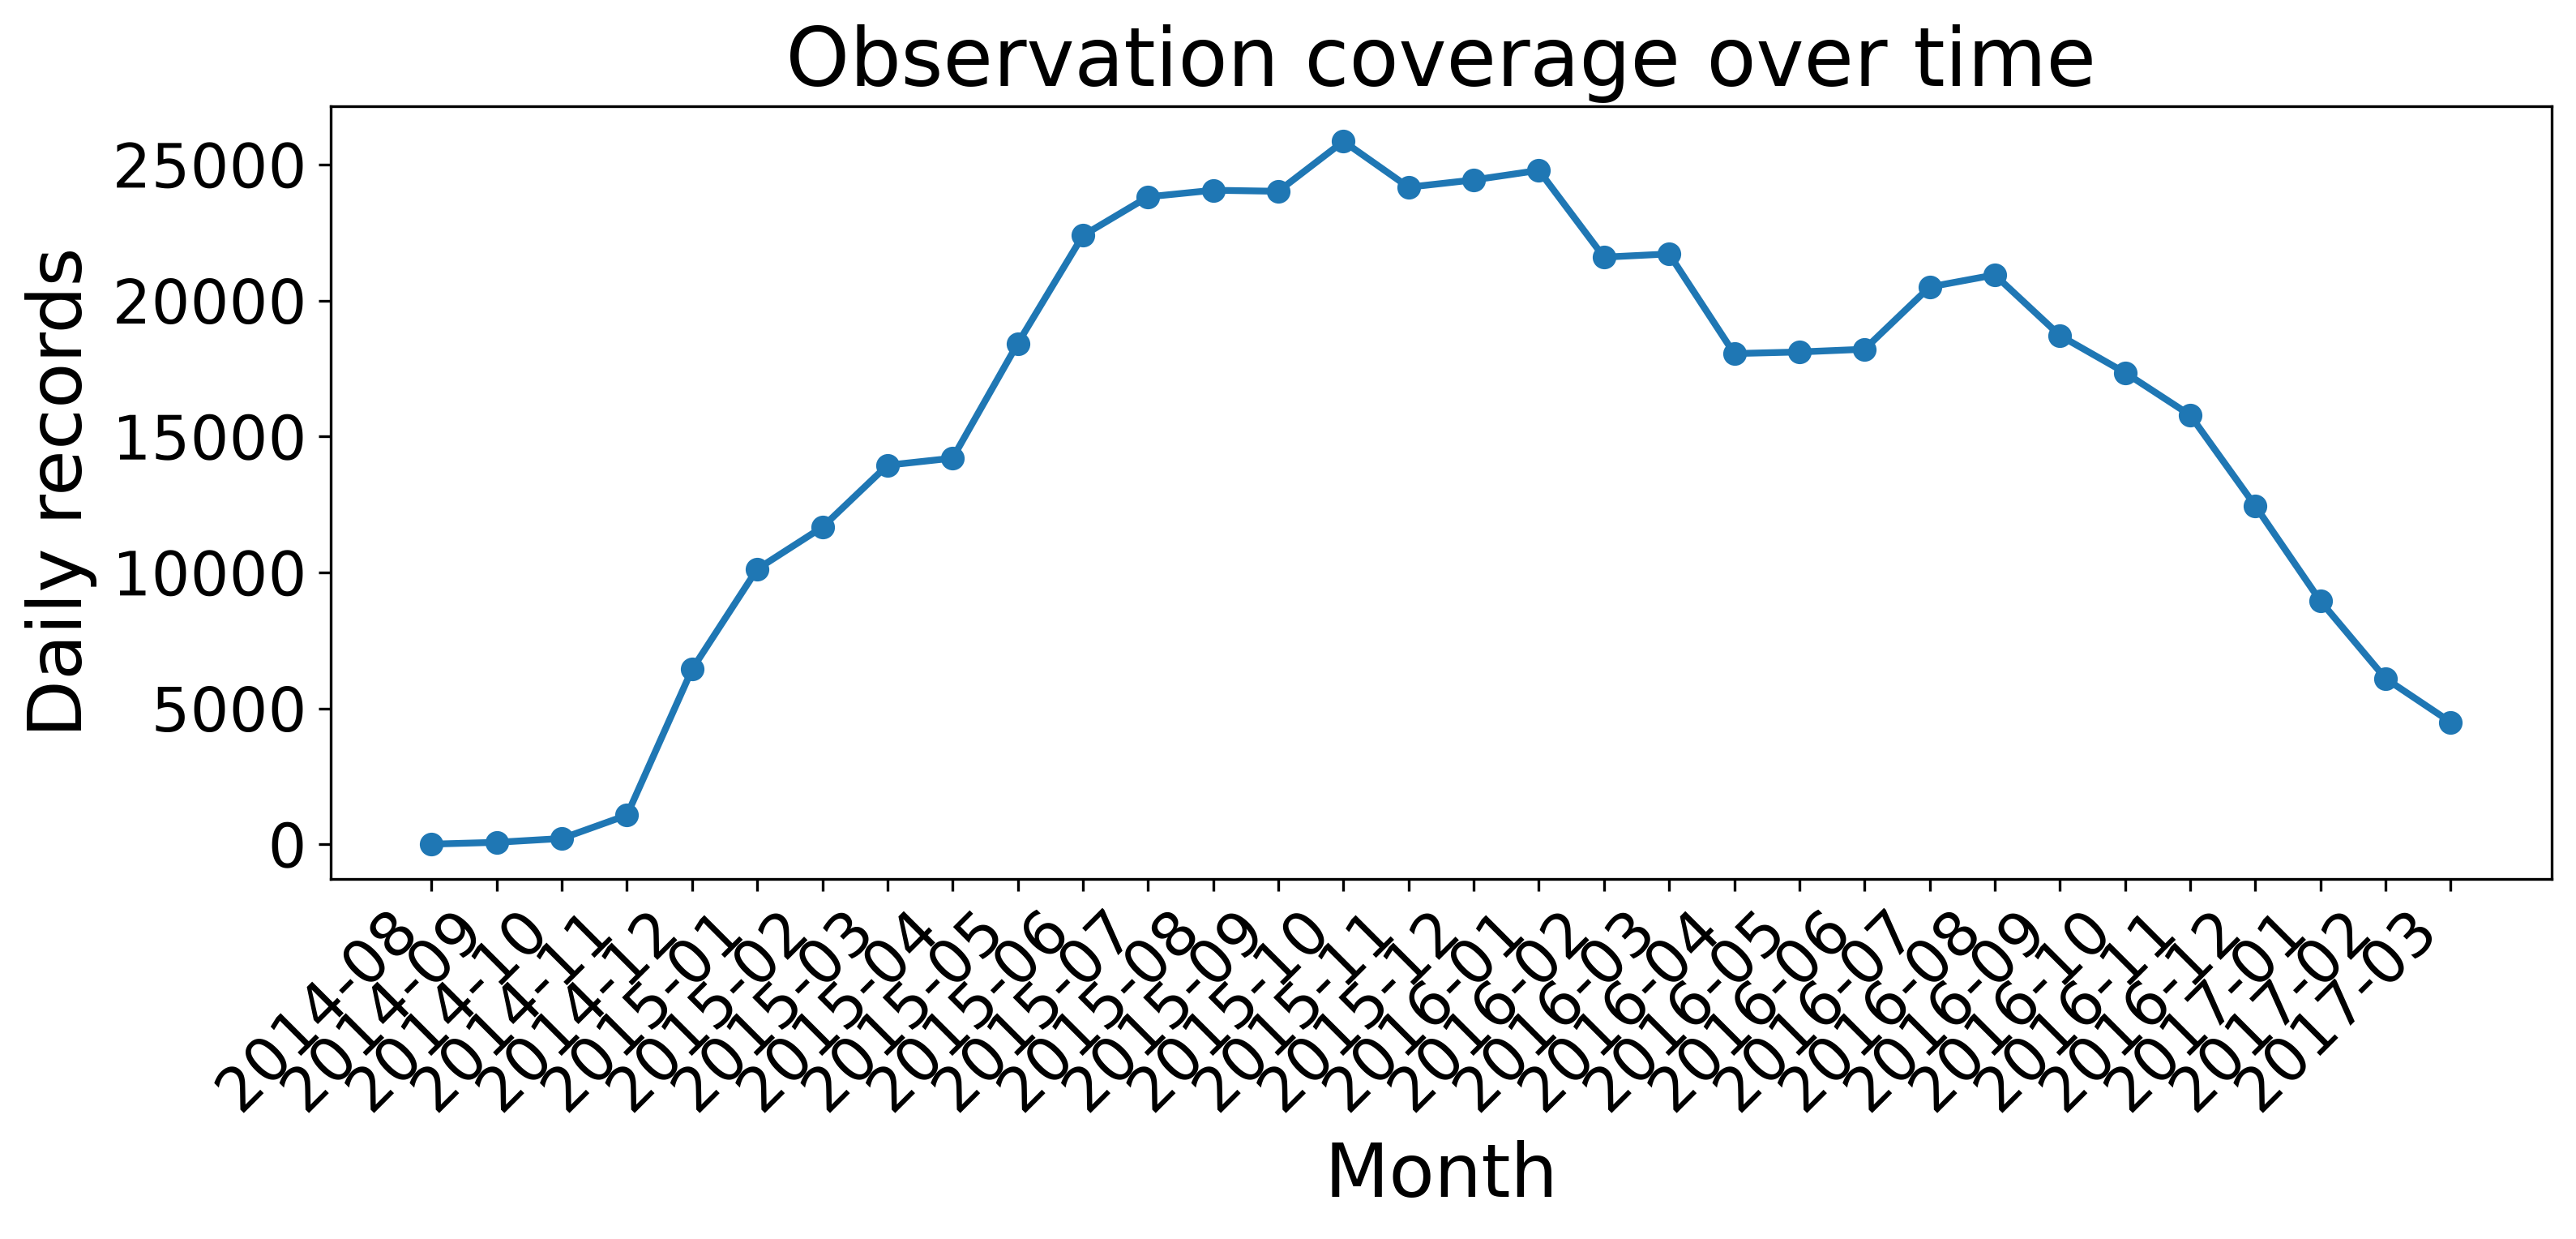
\includegraphics[width=0.66\linewidth]{../outputs/eda/figures/fig06_records_over_time.png}
\end{center}

\end{frame}

%==================== SLIDE 6 ====================
\begin{frame}{Analysis 1.2}

\setbeamercolor{item}{fg=tugreen}
\begin{itemize}
    \item Healthy: 1,547 episodes, 45.21\%
    \item Production disease only: 404 episodes, 11.81\%
    \item Other disease only: 740 episodes, 21.62\%
    \item Production disease + other disease: 731 episodes, 21.36\%
\end{itemize}

\vspace{0.15cm}

\begin{center}
    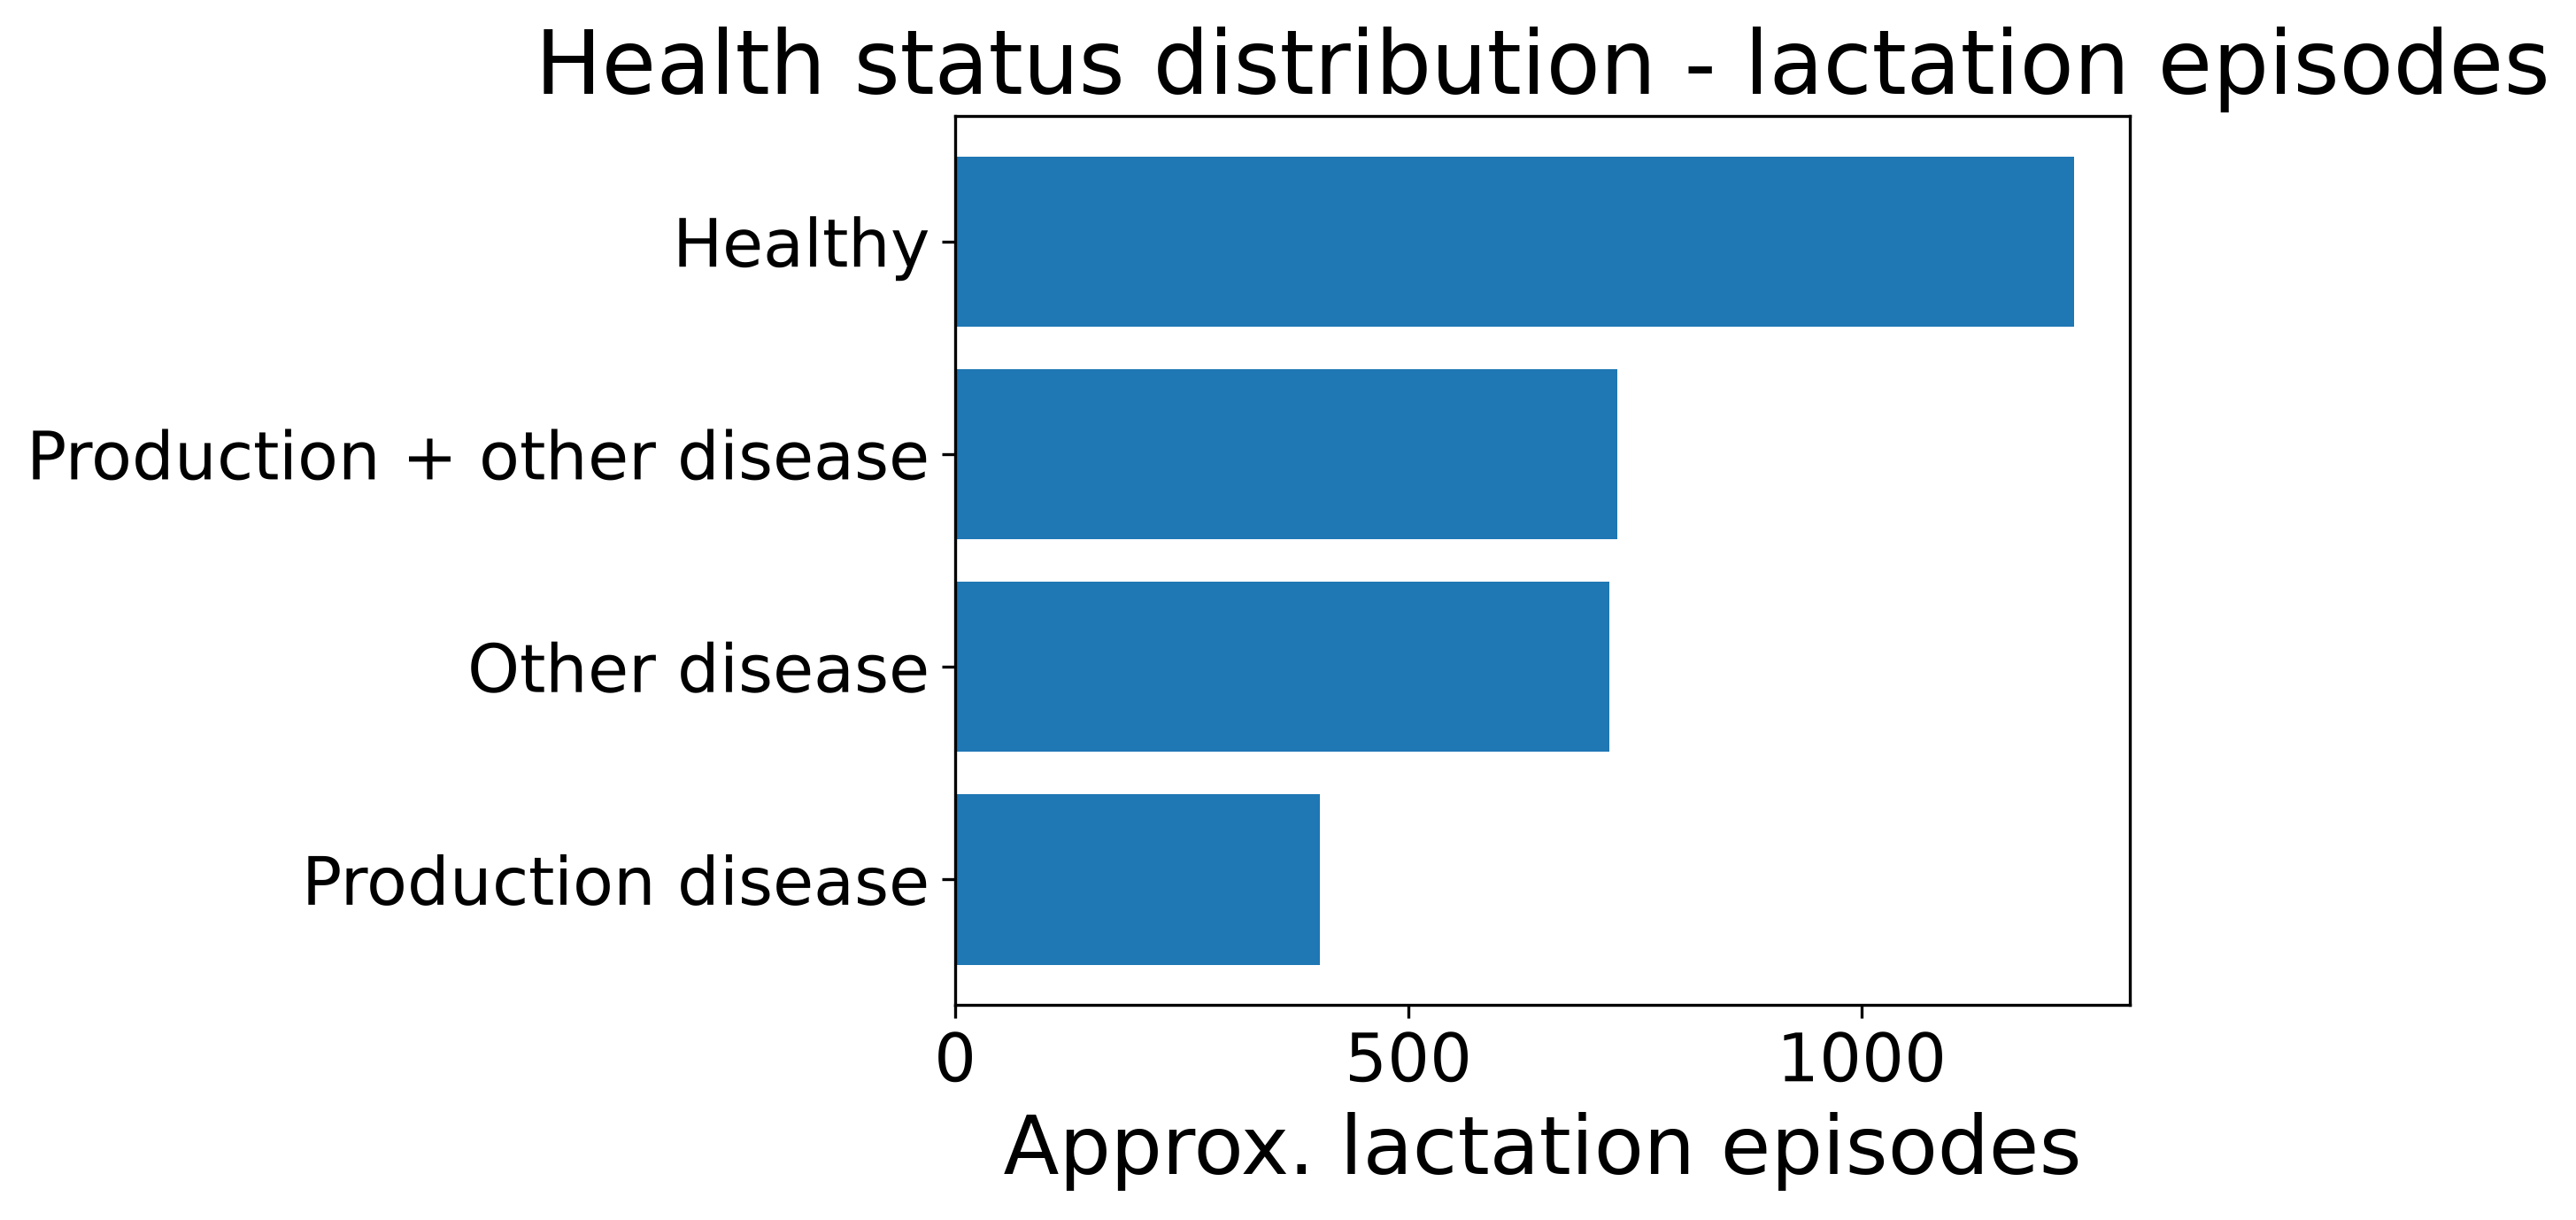
\includegraphics[width=0.58\linewidth]{../outputs/eda/figures/fig02_health_status_lactation_episodes.png}
\end{center}

\end{frame}

%==================== SLIDE 7 ====================
\begin{frame}{Analysis 1.3}

\setbeamercolor{item}{fg=tugreen}
\begin{itemize}
    \item Health-status composition differs across all 12 farms
    \item Farm episode counts range from 84 to 722 episodes
    \item The largest farm has about 8.6 times more episodes than the smallest farm
\end{itemize}

\vspace{0.10cm}

\begin{center}
    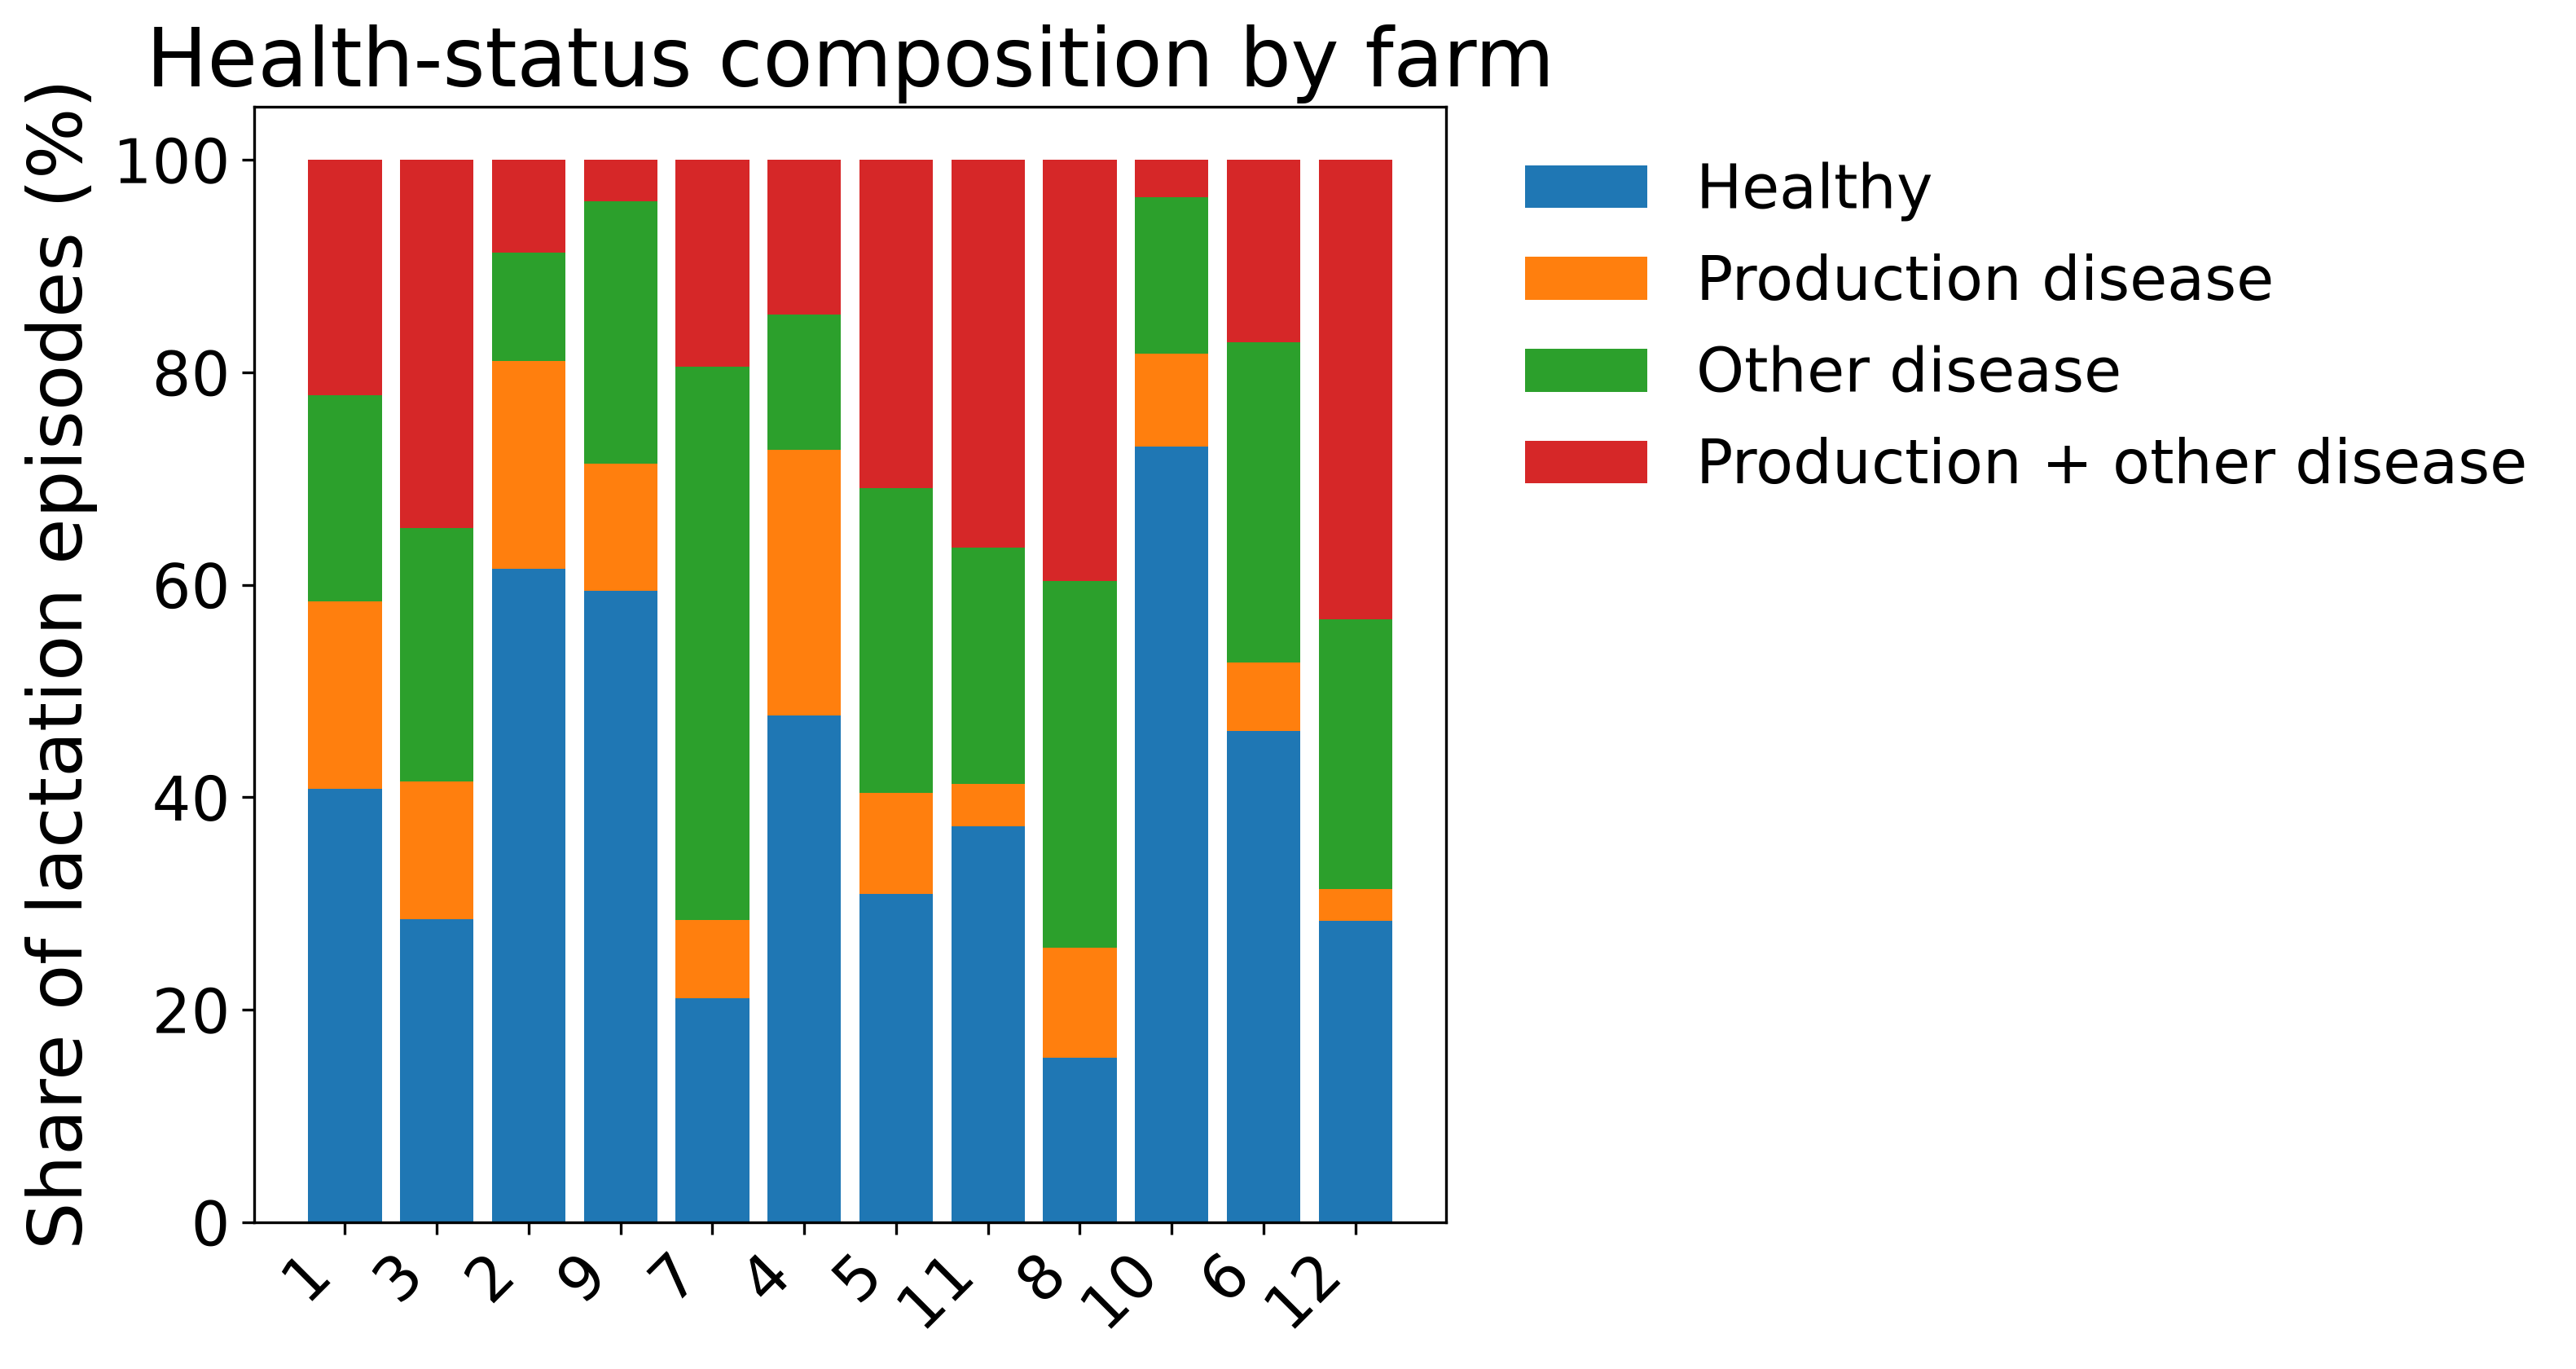
\includegraphics[width=0.58\linewidth]{../outputs/eda/figures/fig17_health_status_by_farm_percent.png}
\end{center}

\end{frame}

%==================== SLIDE 8 ====================
\begin{frame}{Analysis 1.4}

\setbeamercolor{item}{fg=tugreen}
\begin{itemize}
    \item Top diagnosis: septic claw/hoof disease with 700 event rows
    \item Mastitis: 578 event rows
    \item Parasitic disease: 562 event rows
    \item Top 4 diagnoses together account for 2,285 event rows
\end{itemize}

\vspace{0.10cm}

\begin{center}
    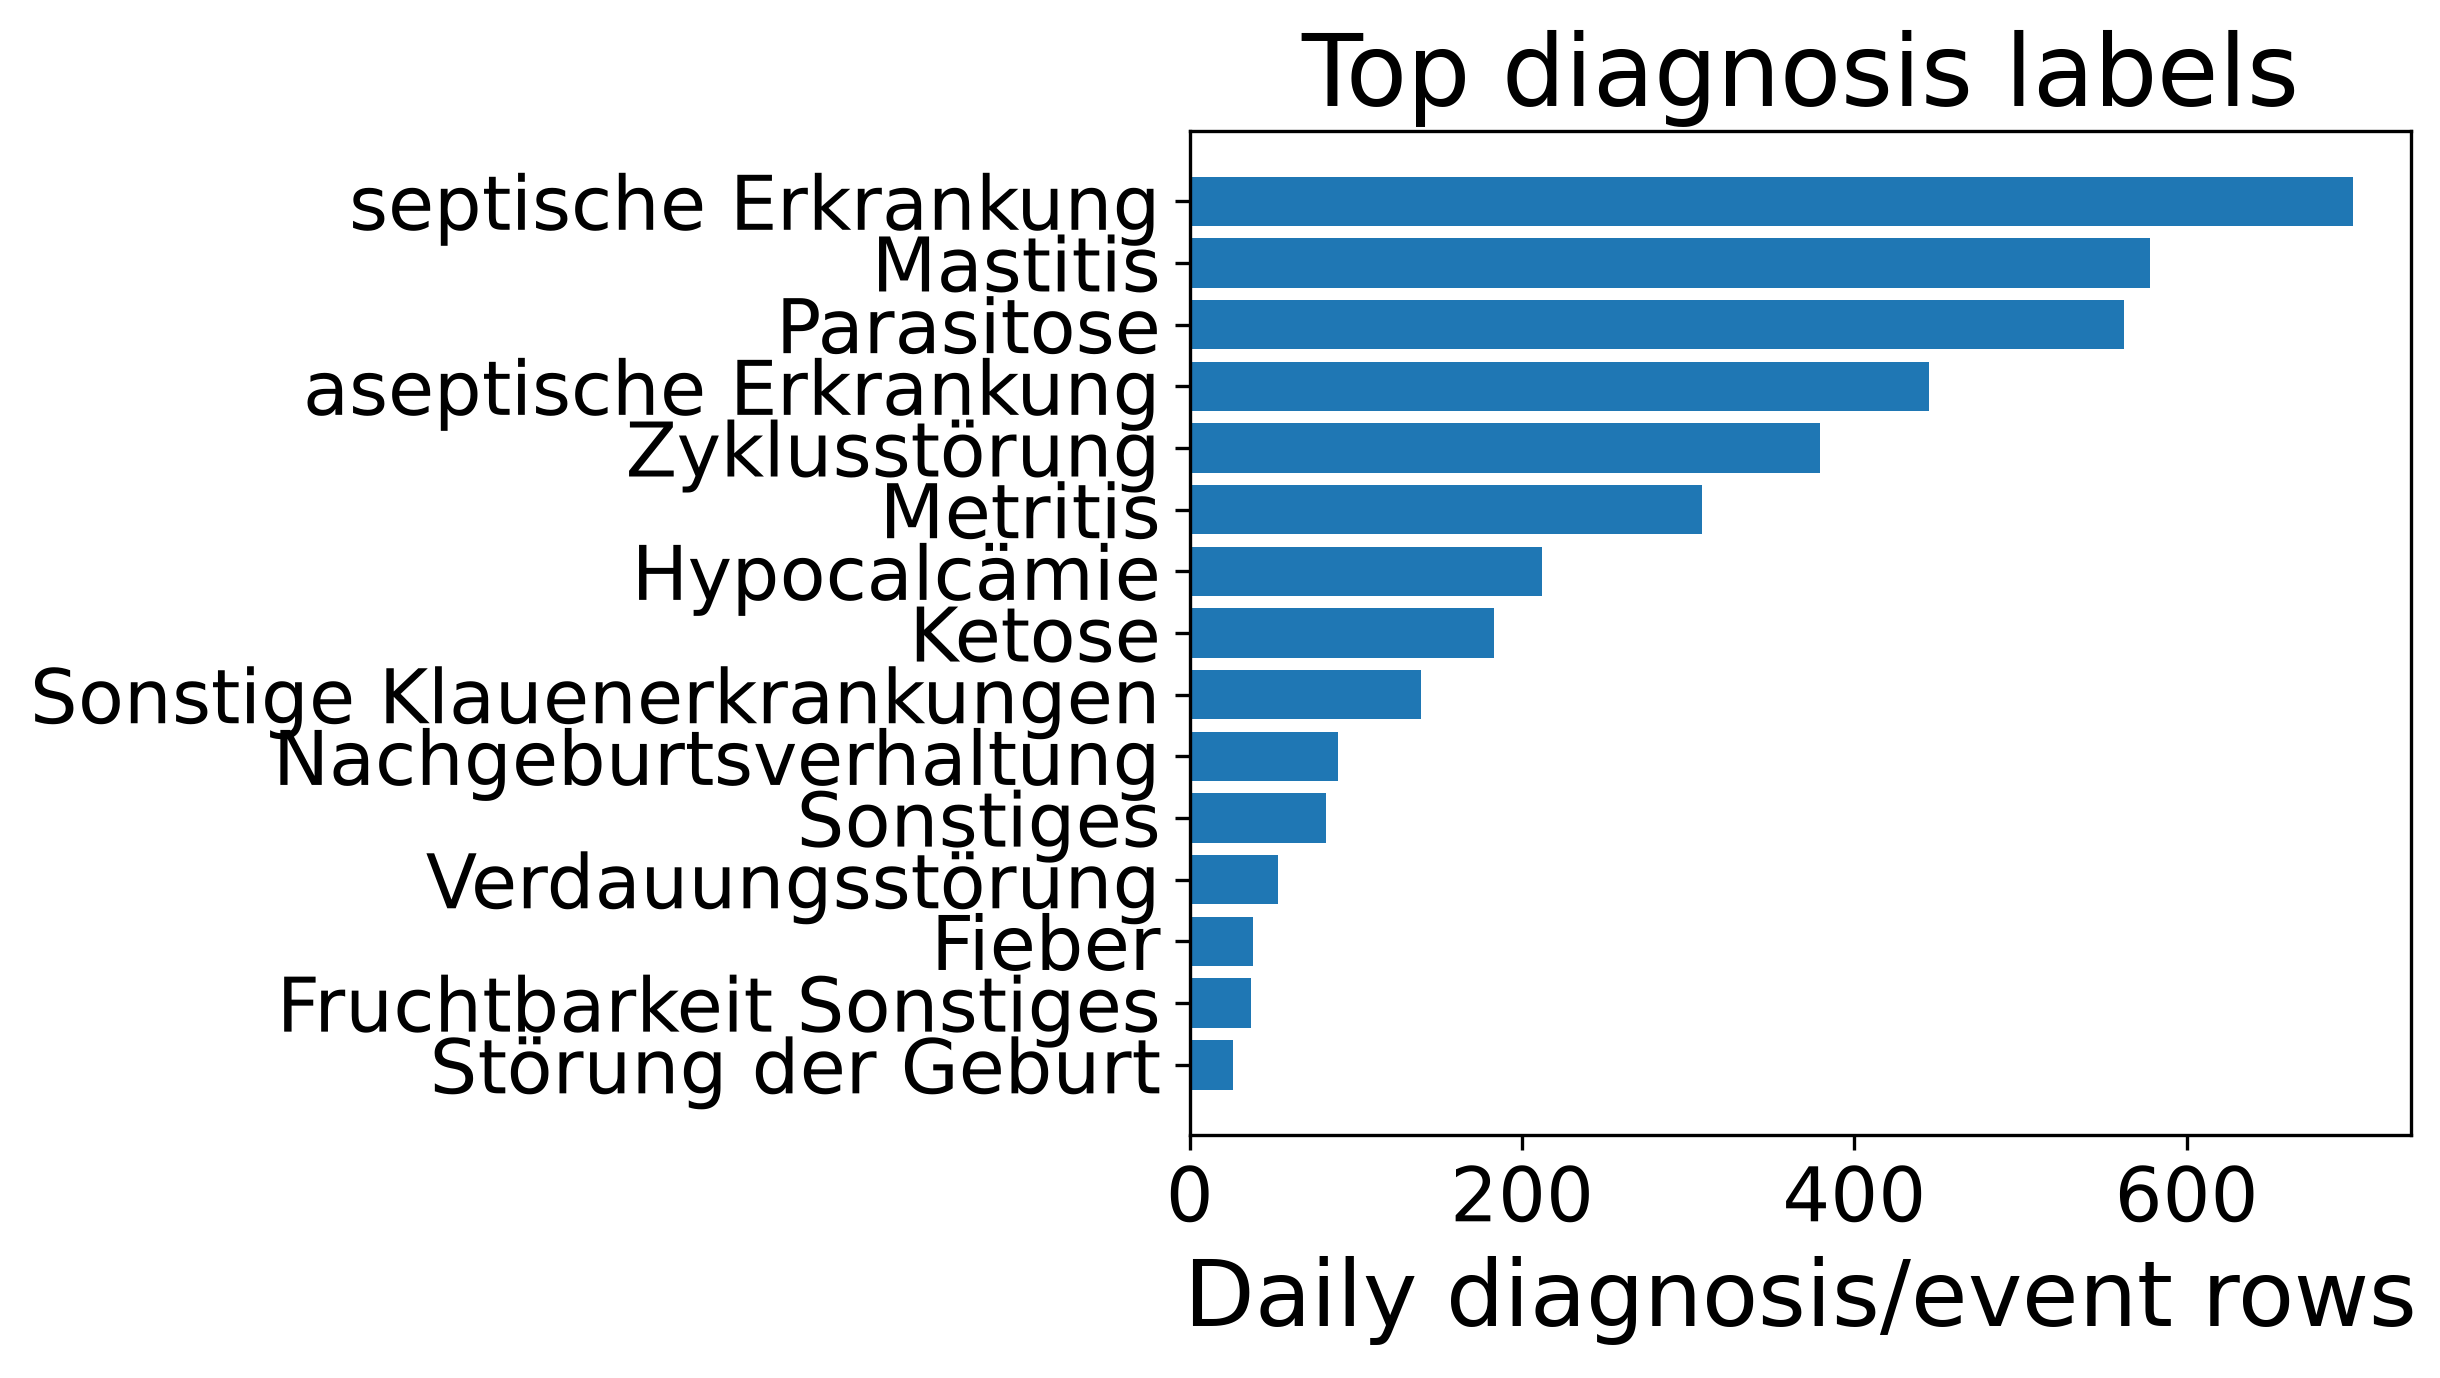
\includegraphics[width=0.62\linewidth]{../outputs/eda/figures/fig11_top_diagnoses.png}
\end{center}

\end{frame}

%==================== SLIDE 9 ====================
\begin{frame}{Analysis 1.5}

\setbeamercolor{item}{fg=tugreen}
\begin{itemize}
    \item Breed groups show different health-status distributions
    \item German Holstein is the dominant breed group
    \item Smaller breed groups have fewer lactation episodes and should be interpreted carefully
    \item Breed should be retained as a grouping variable in future analysis
\end{itemize}

\vspace{0.15cm}

\begin{center}
    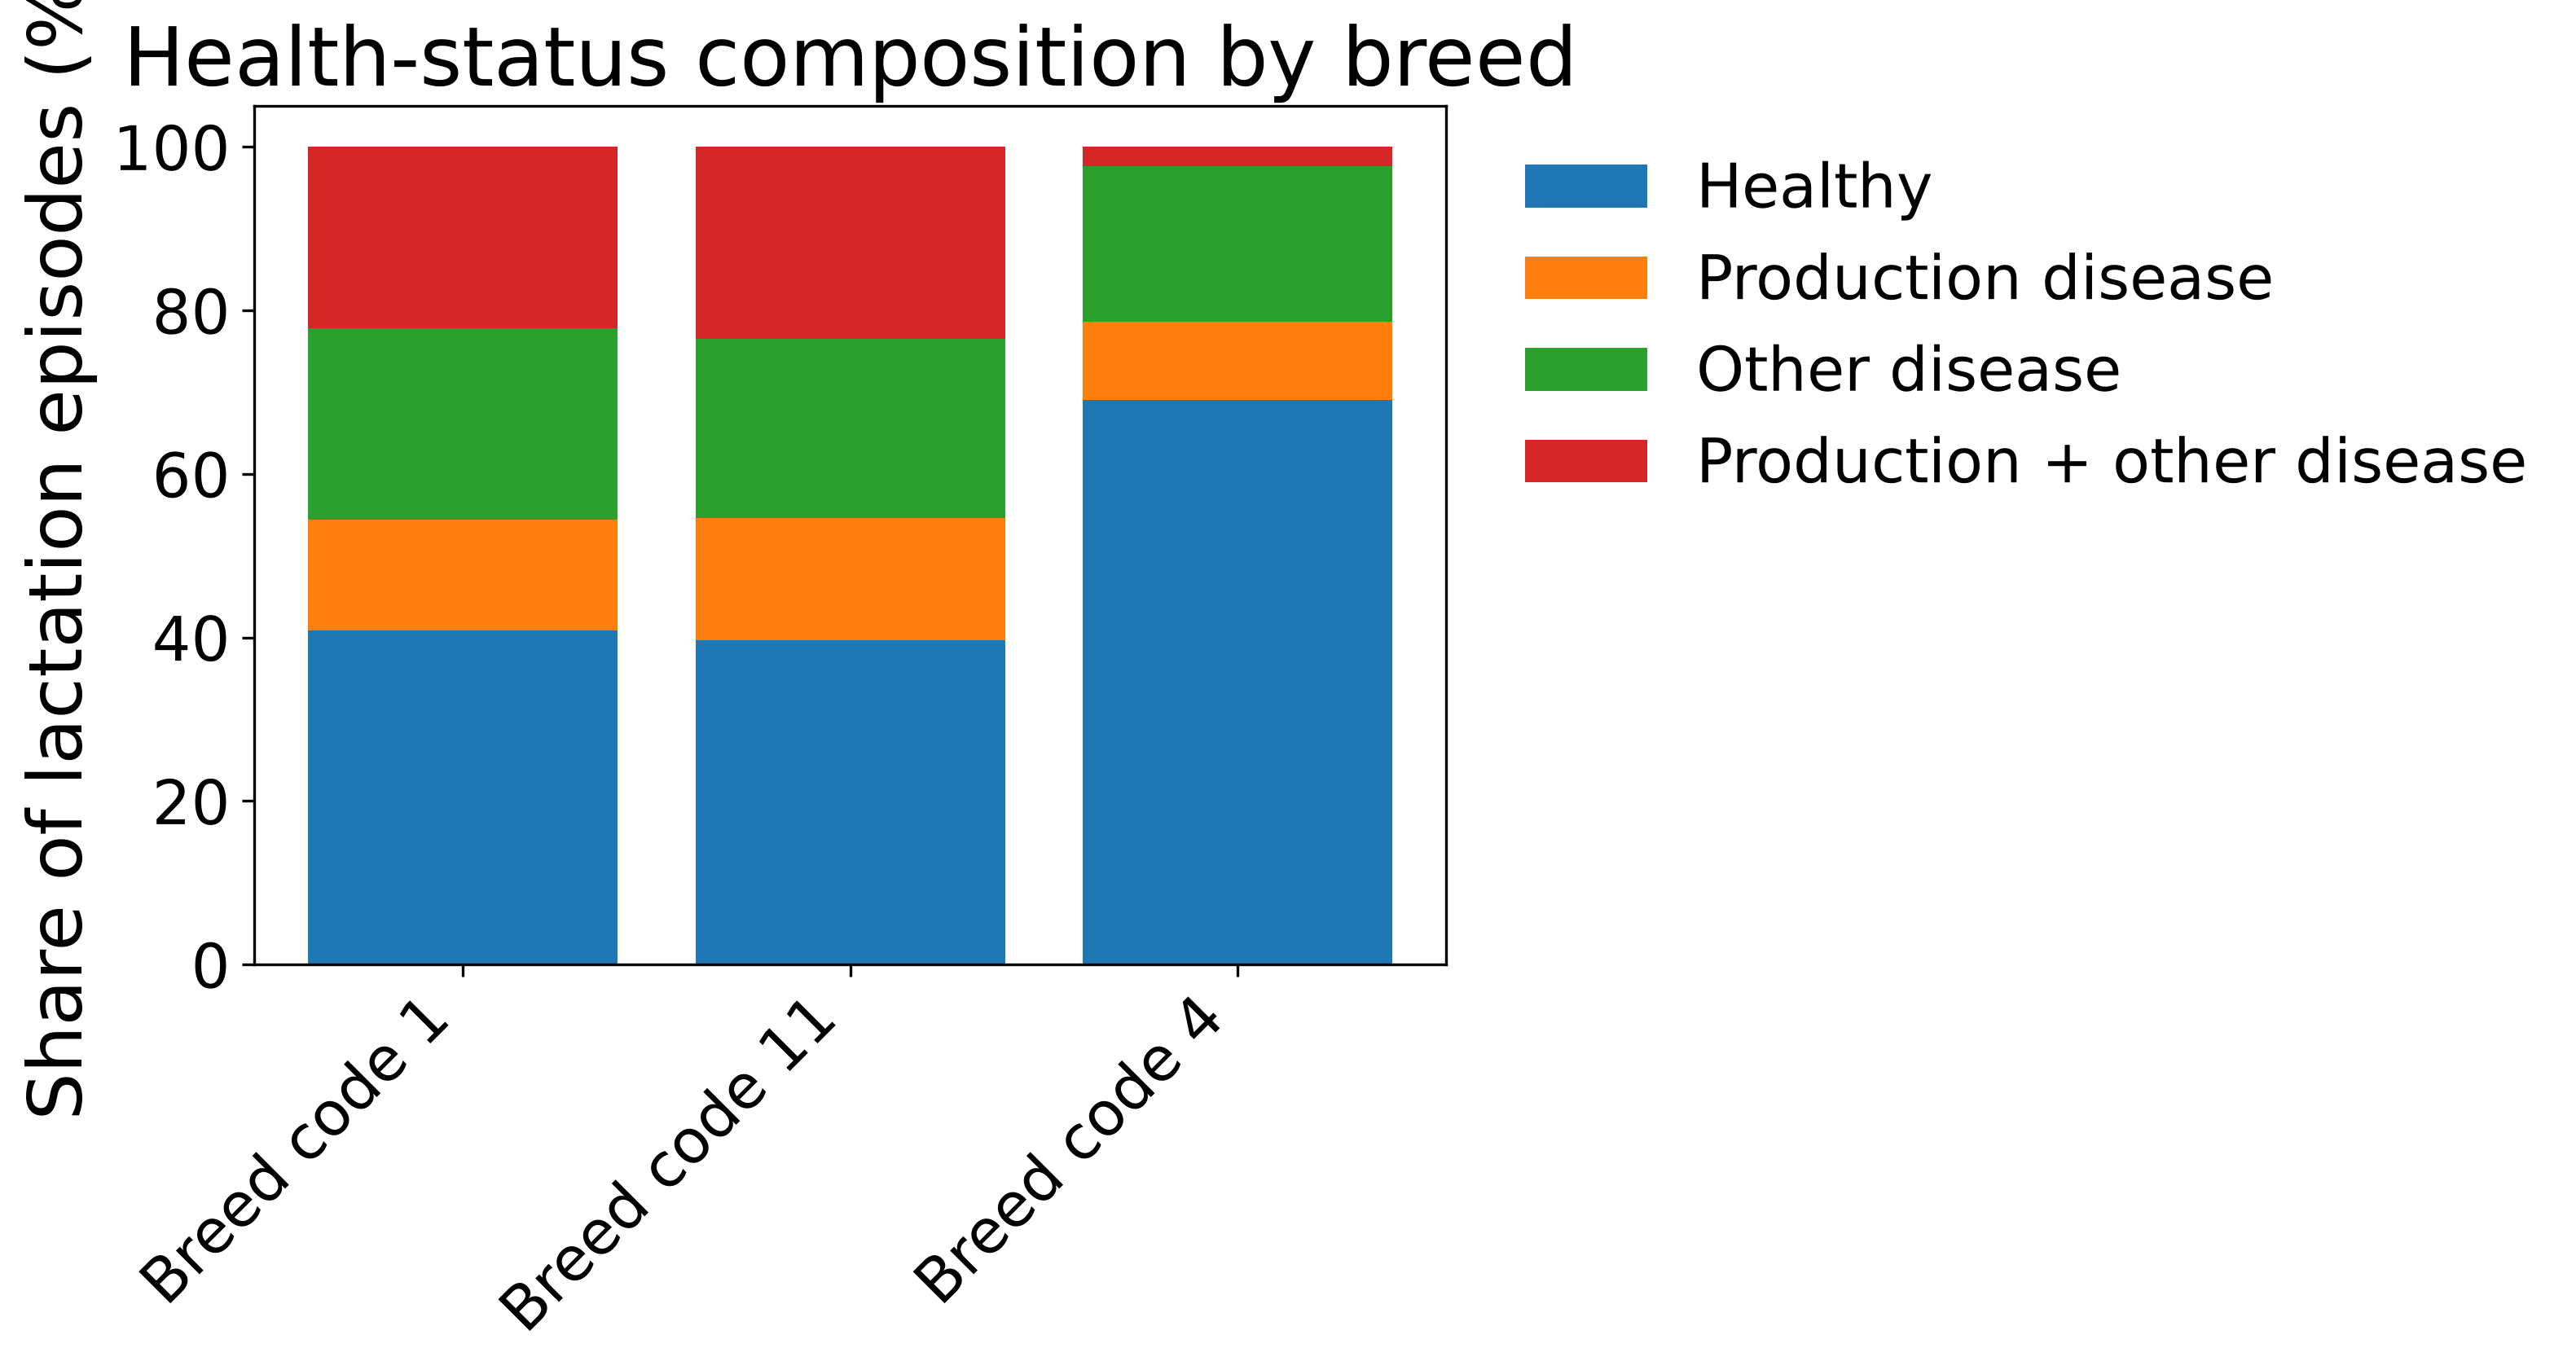
\includegraphics[width=0.58\linewidth]{../outputs/eda/figures/fig18_health_status_by_breed_percent.png}
\end{center}

\end{frame}

%==================== SLIDE 10 ====================
\begin{frame}{Analysis 1.6}

\setbeamercolor{item}{fg=tugreen}
\begin{itemize}
    \item Milk yield is missing in 13.98\% of daily records
    \item Body condition score is missing in 96.22\% of daily records
    \item BHB, NEFA and glucose are missing in about 98.53\% of daily records
    \item Missingness mainly reflects different measurement schedules
\end{itemize}

\vspace{0.15cm}

\begin{center}
    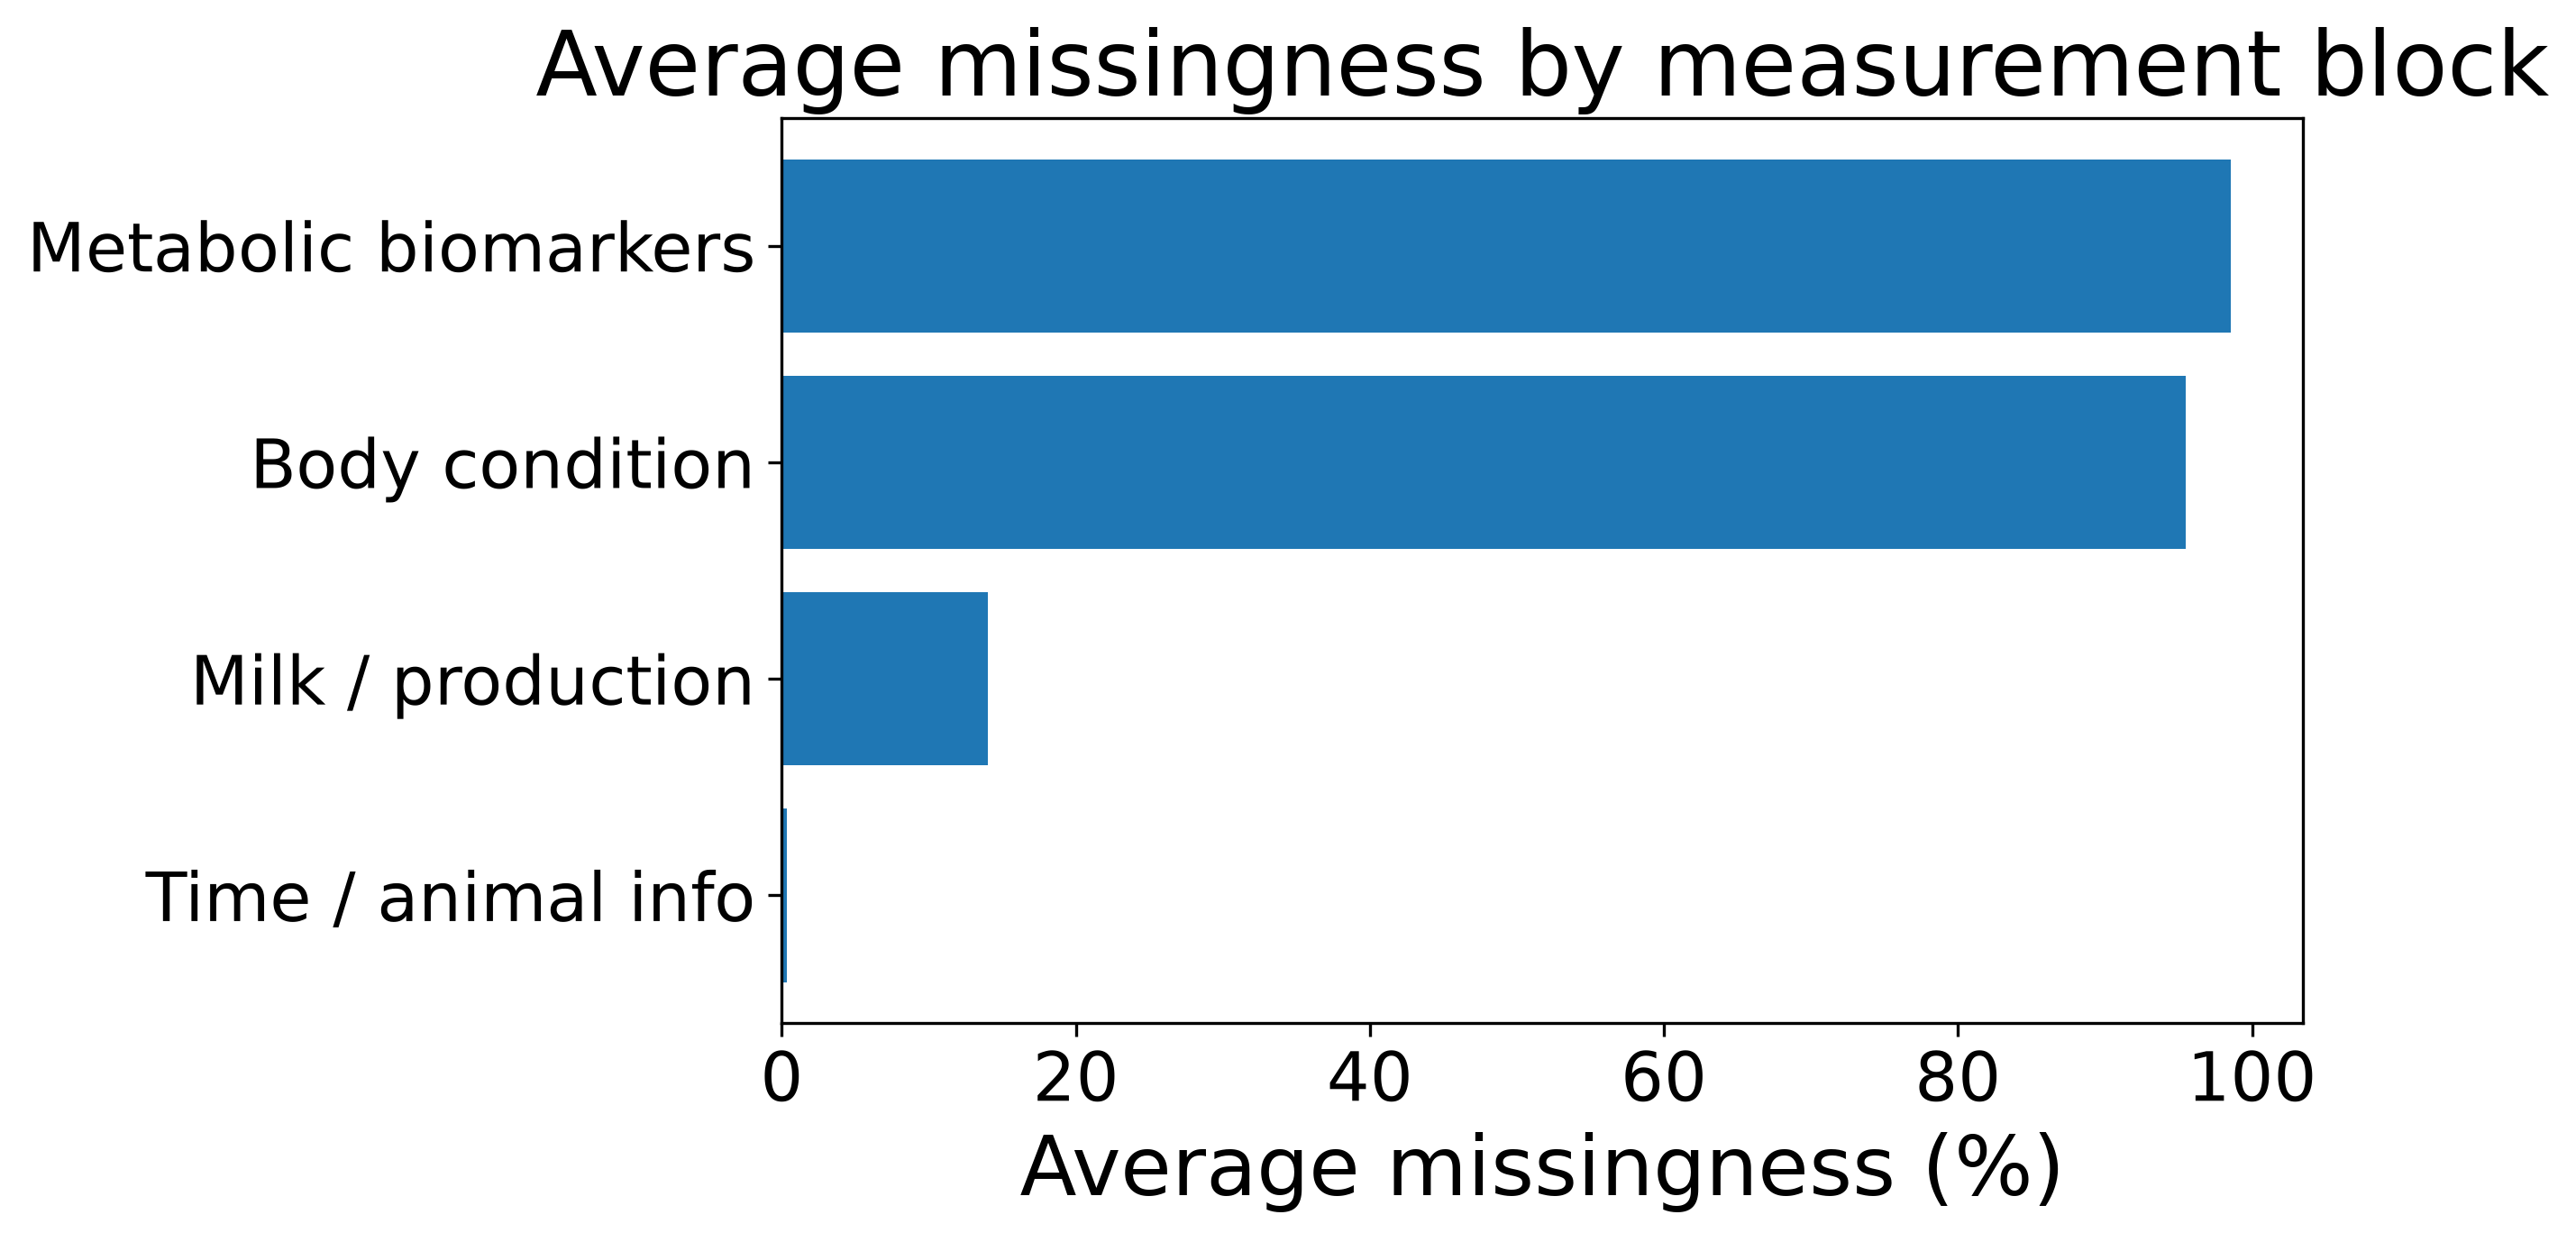
\includegraphics[width=0.62\linewidth]{../outputs/eda/figures/fig29_missingness_by_measurement_block.png}
\end{center}

\end{frame}

%==================== SLIDE 11 ====================
\begin{frame}{Analysis 1.7}

\setbeamercolor{item}{fg=tugreen}
\begin{itemize}
    \item Milk yield is available in 423,673 daily records
    \item Overall median milk yield is 32.45 kg
    \item Median milk yield differs by health status
    \item Lowest and highest health-status medians differ by about 2.14 kg
\end{itemize}

\vspace{0.10cm}

\begin{center}
    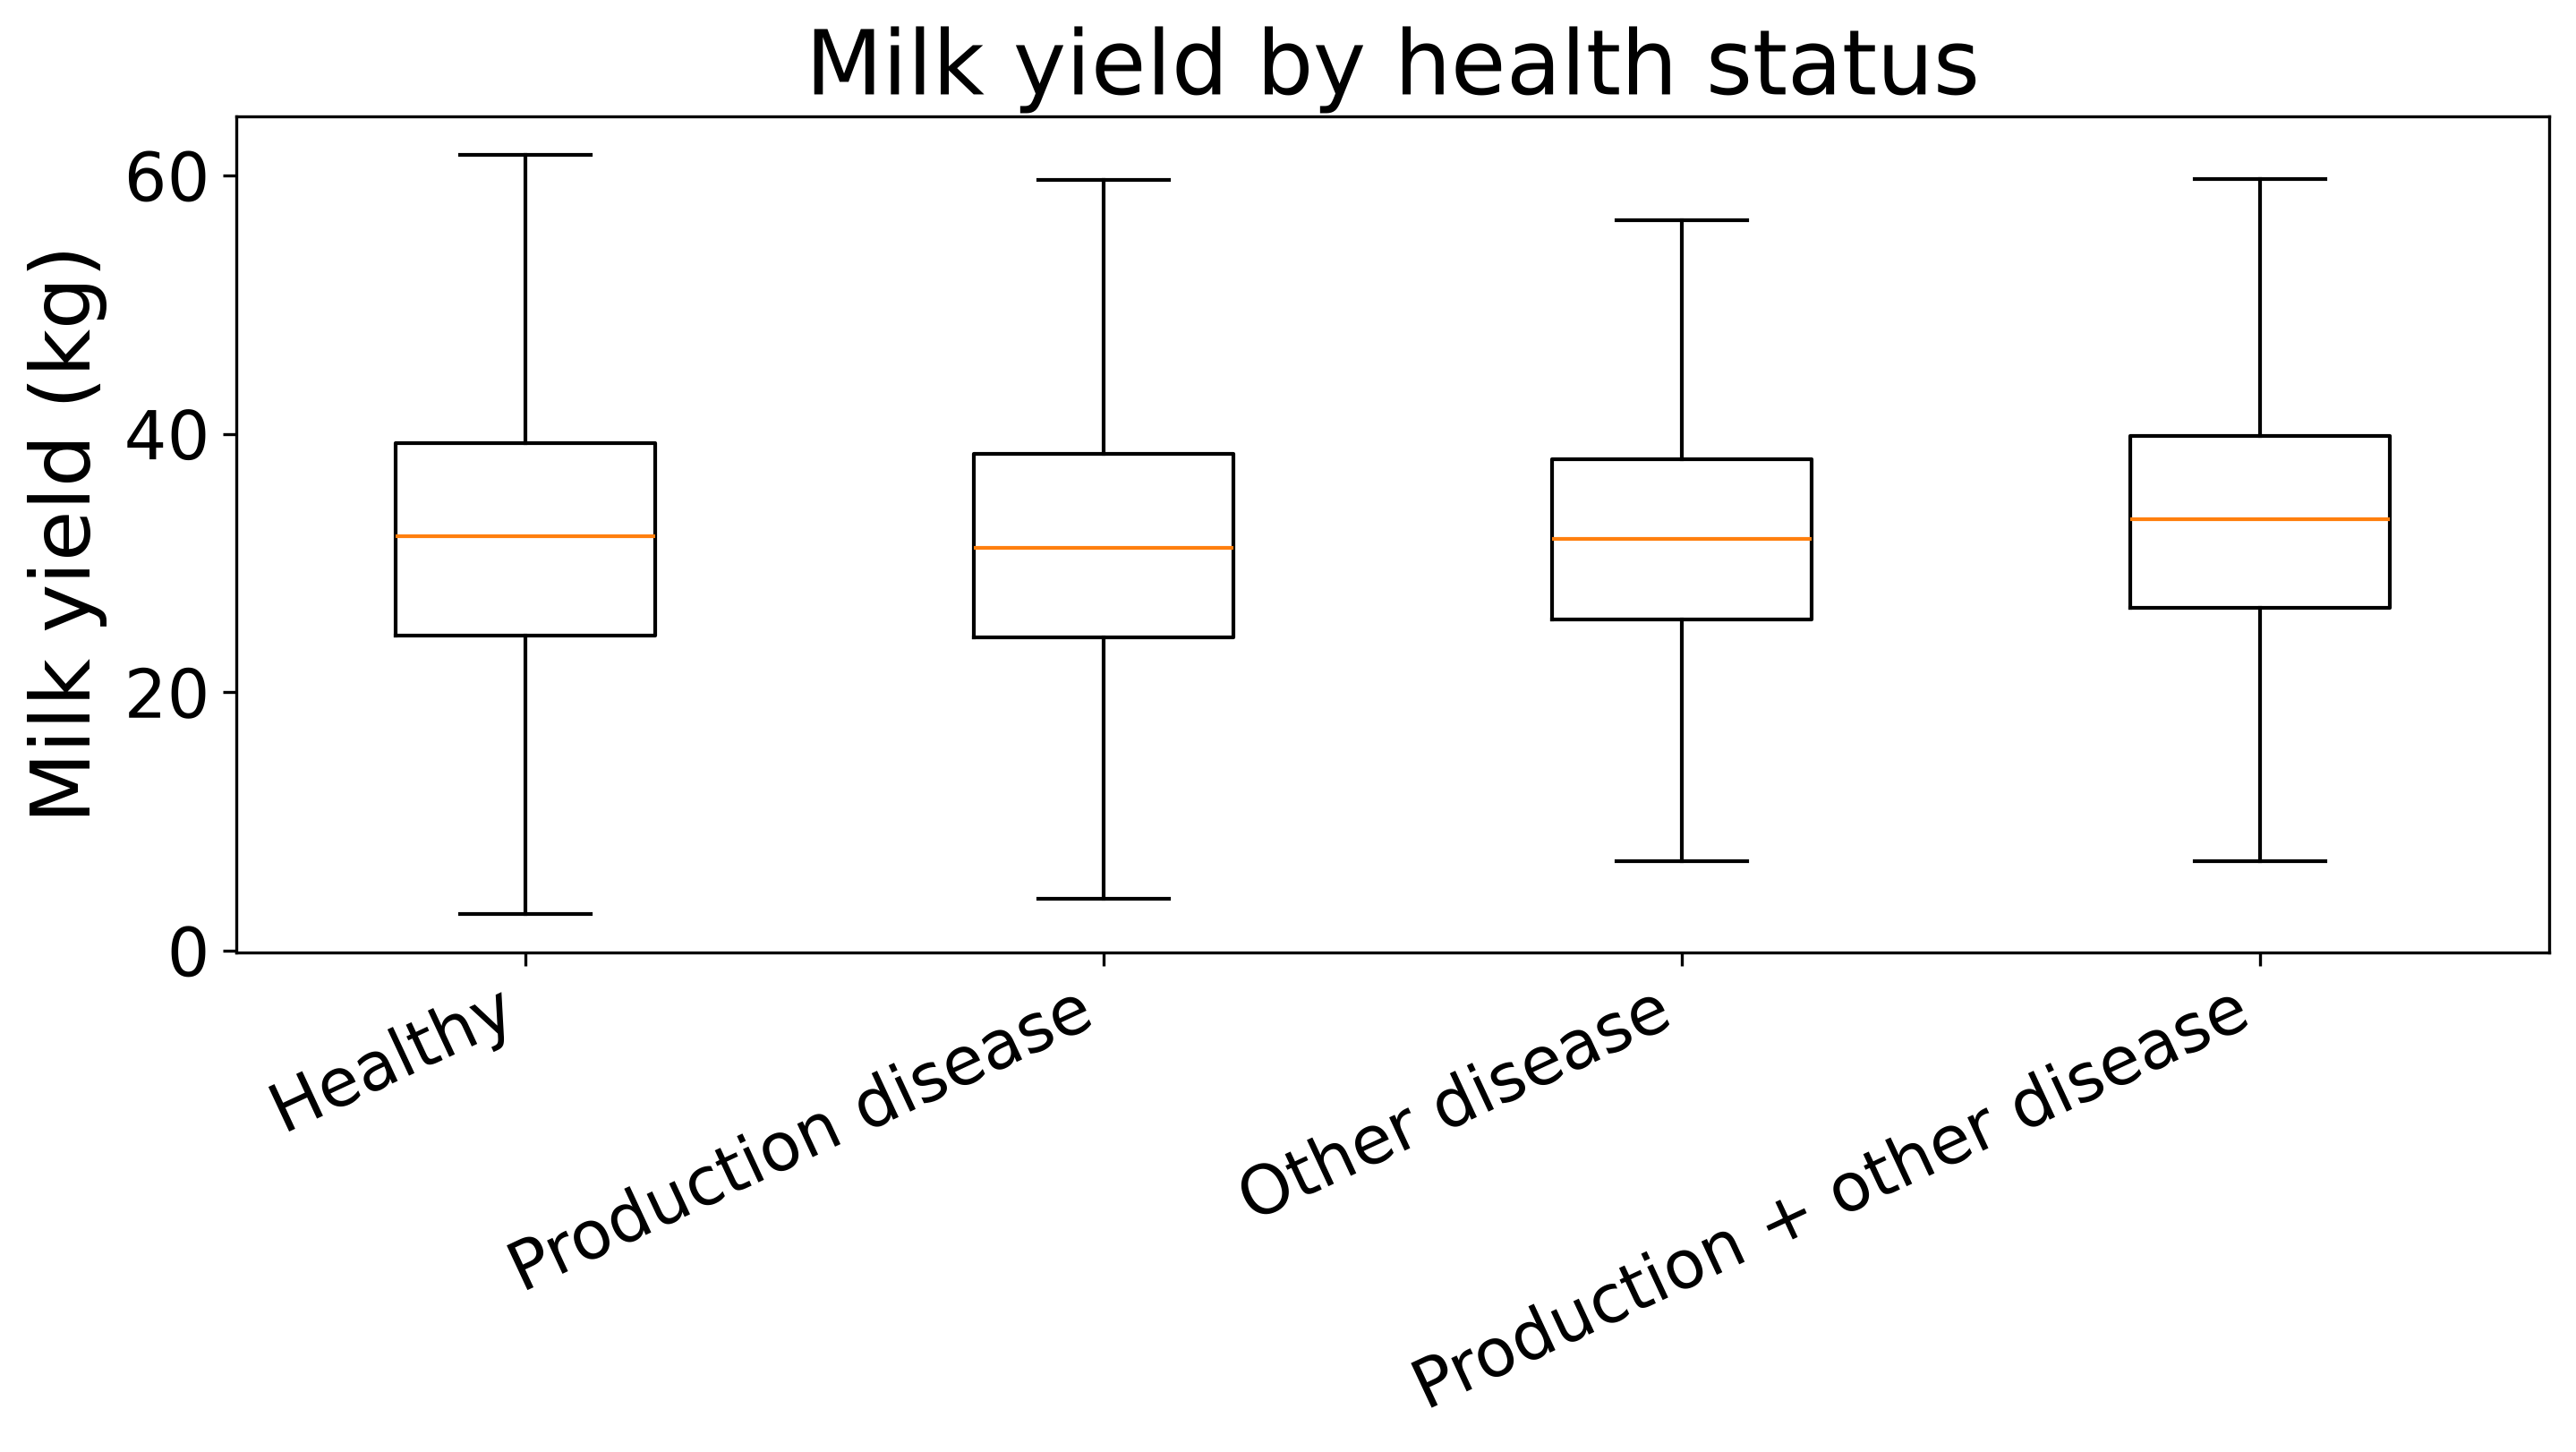
\includegraphics[width=0.62\linewidth]{../outputs/eda/figures/fig13_milk_yield_by_health_status.png}
\end{center}

\end{frame}

%==================== SLIDE 12 ====================
\begin{frame}{Analysis 1.8}

\setbeamercolor{item}{fg=tugreen}
\begin{itemize}
    \item Milk yield changes across days-in-milk bins
    \item The time trend differs between health-status groups
    \item Days in milk should be considered in feature engineering
    \item Raw milk yield should not be interpreted without lactation-stage context
\end{itemize}

\vspace{0.10cm}

\begin{center}
    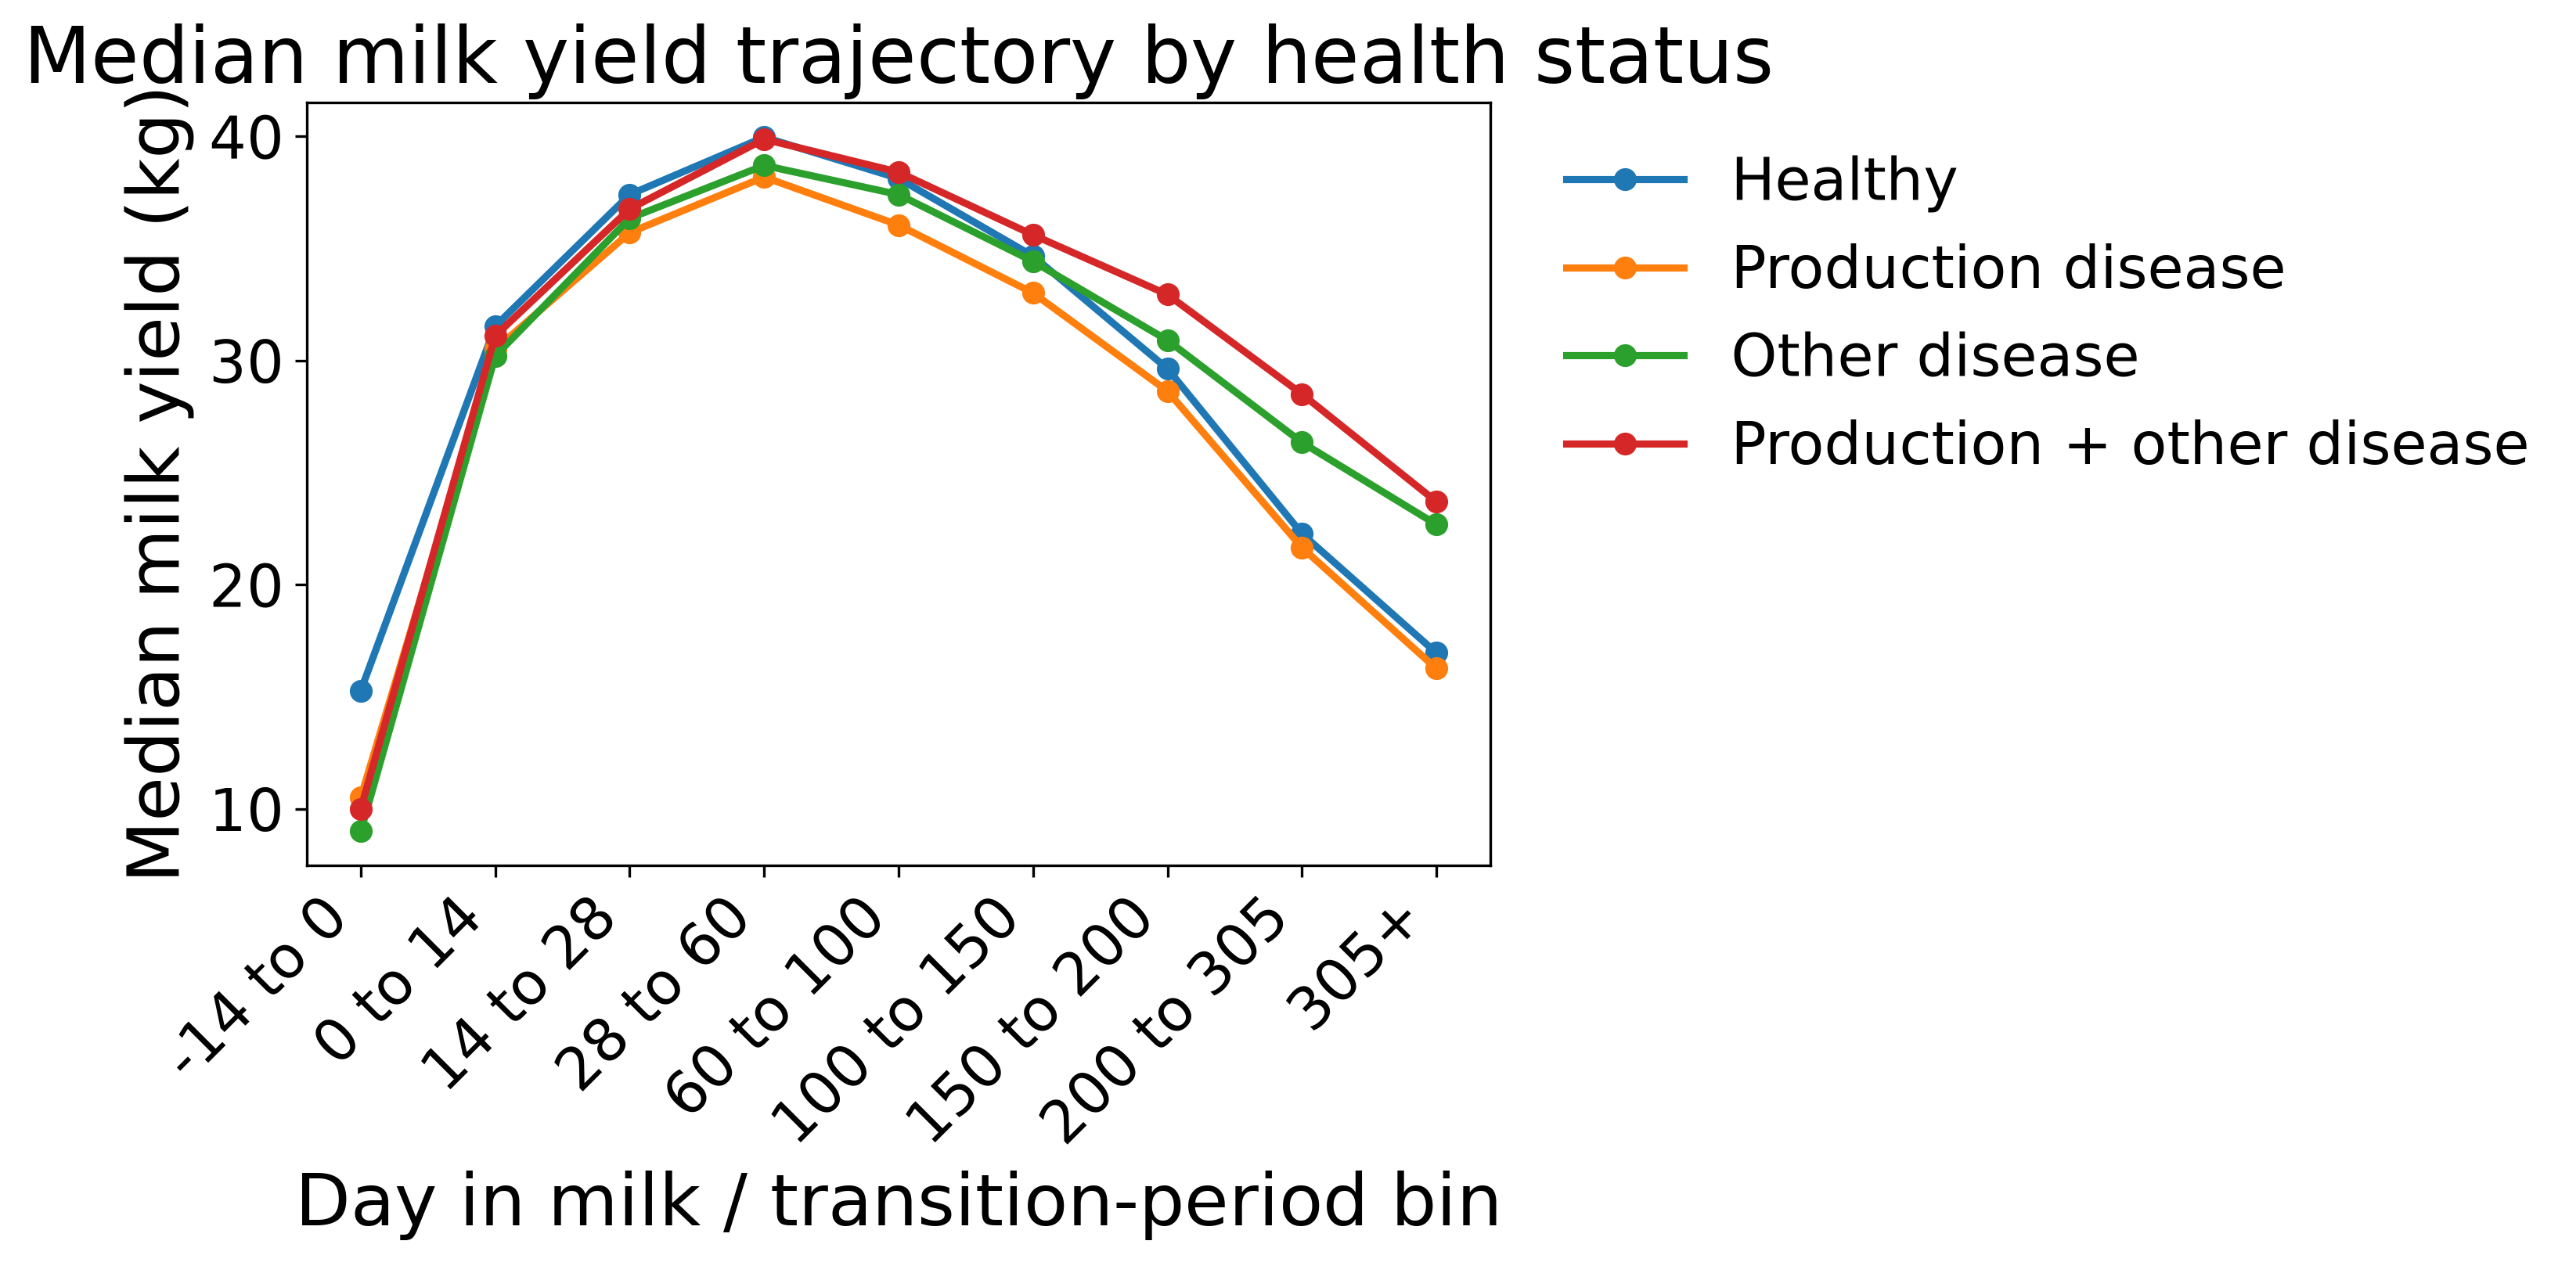
\includegraphics[width=0.62\linewidth]{../outputs/eda/figures/fig23_milk_yield_dim_trend_by_health_status.png}
\end{center}

\end{frame}

%==================== SLIDE 13 ====================
\begin{frame}{Analysis 1.9}

\setbeamercolor{item}{fg=tugreen}
\begin{itemize}
    \item BHB above about 1.2 mmol/L is commonly used as a subclinical ketosis warning threshold
    \item NEFA above about 0.7 mmol/L after calving can indicate excessive fat mobilization
    \item Both markers are linked to negative energy balance in early lactation
    \item Interpretation depends strongly on sampling time around calving
\end{itemize}

\vspace{0.10cm}

\begin{columns}[T,totalwidth=\textwidth]
\column{0.50\textwidth}
\begin{center}
    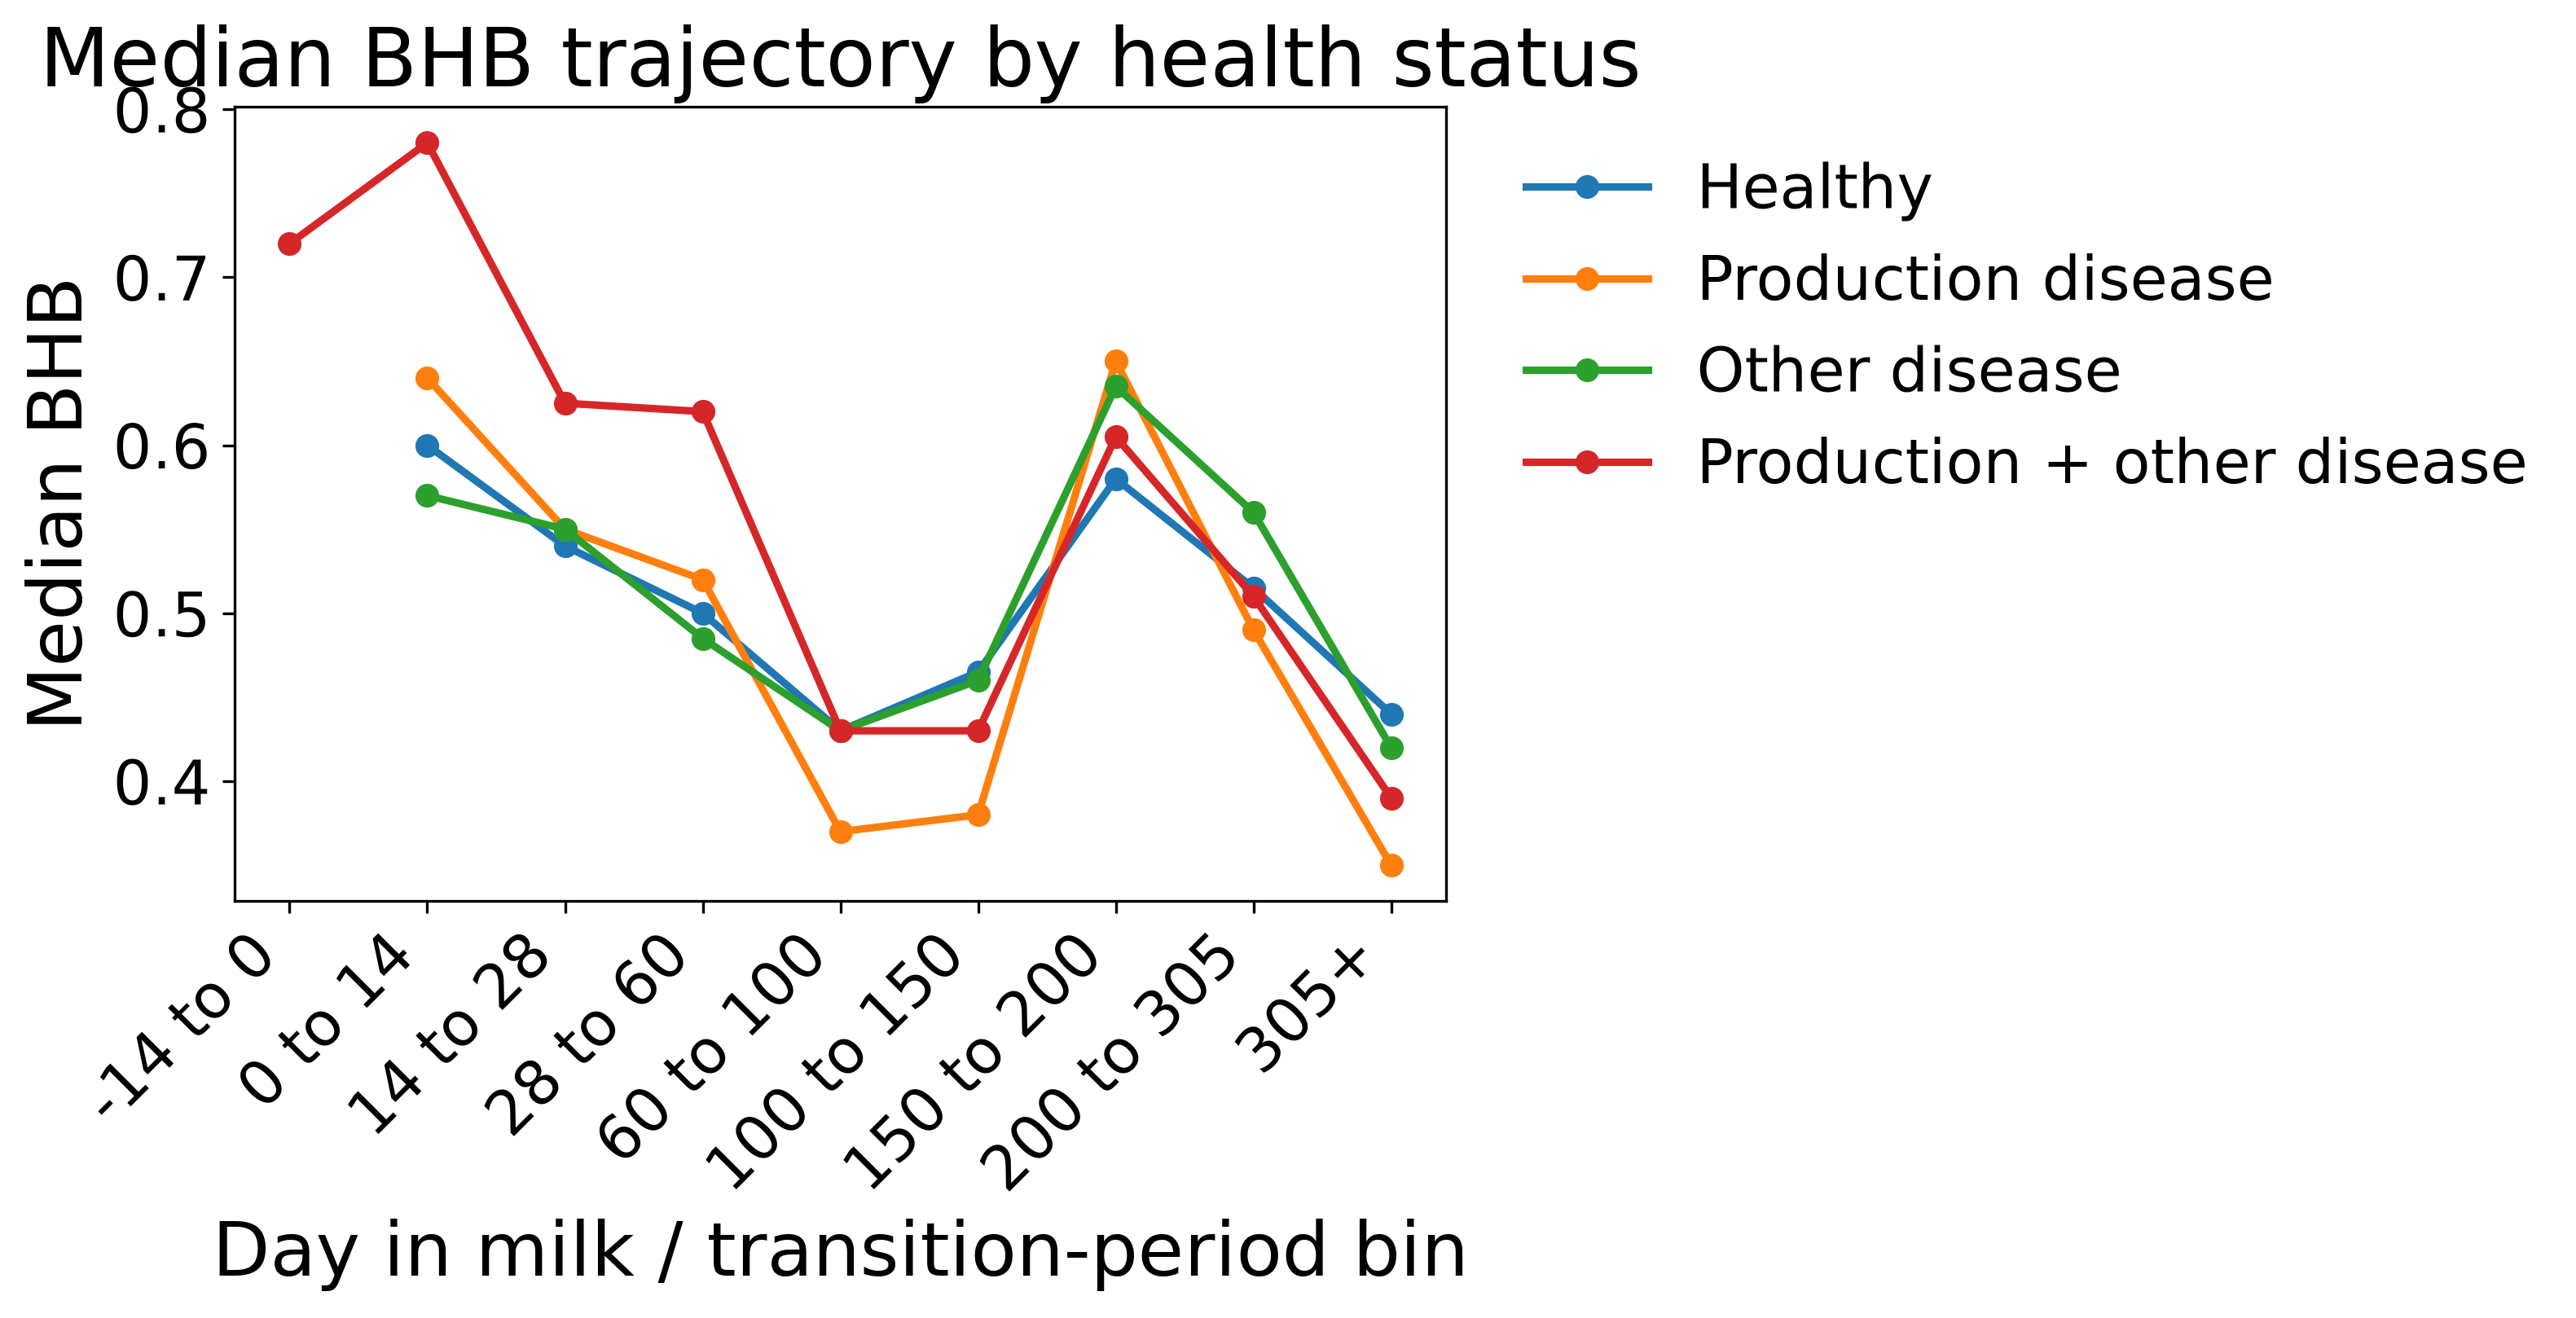
\includegraphics[width=0.95\linewidth]{../outputs/eda/figures/fig24_bhb_dim_trend_by_health_status.png}
\end{center}

\column{0.50\textwidth}
\begin{center}
    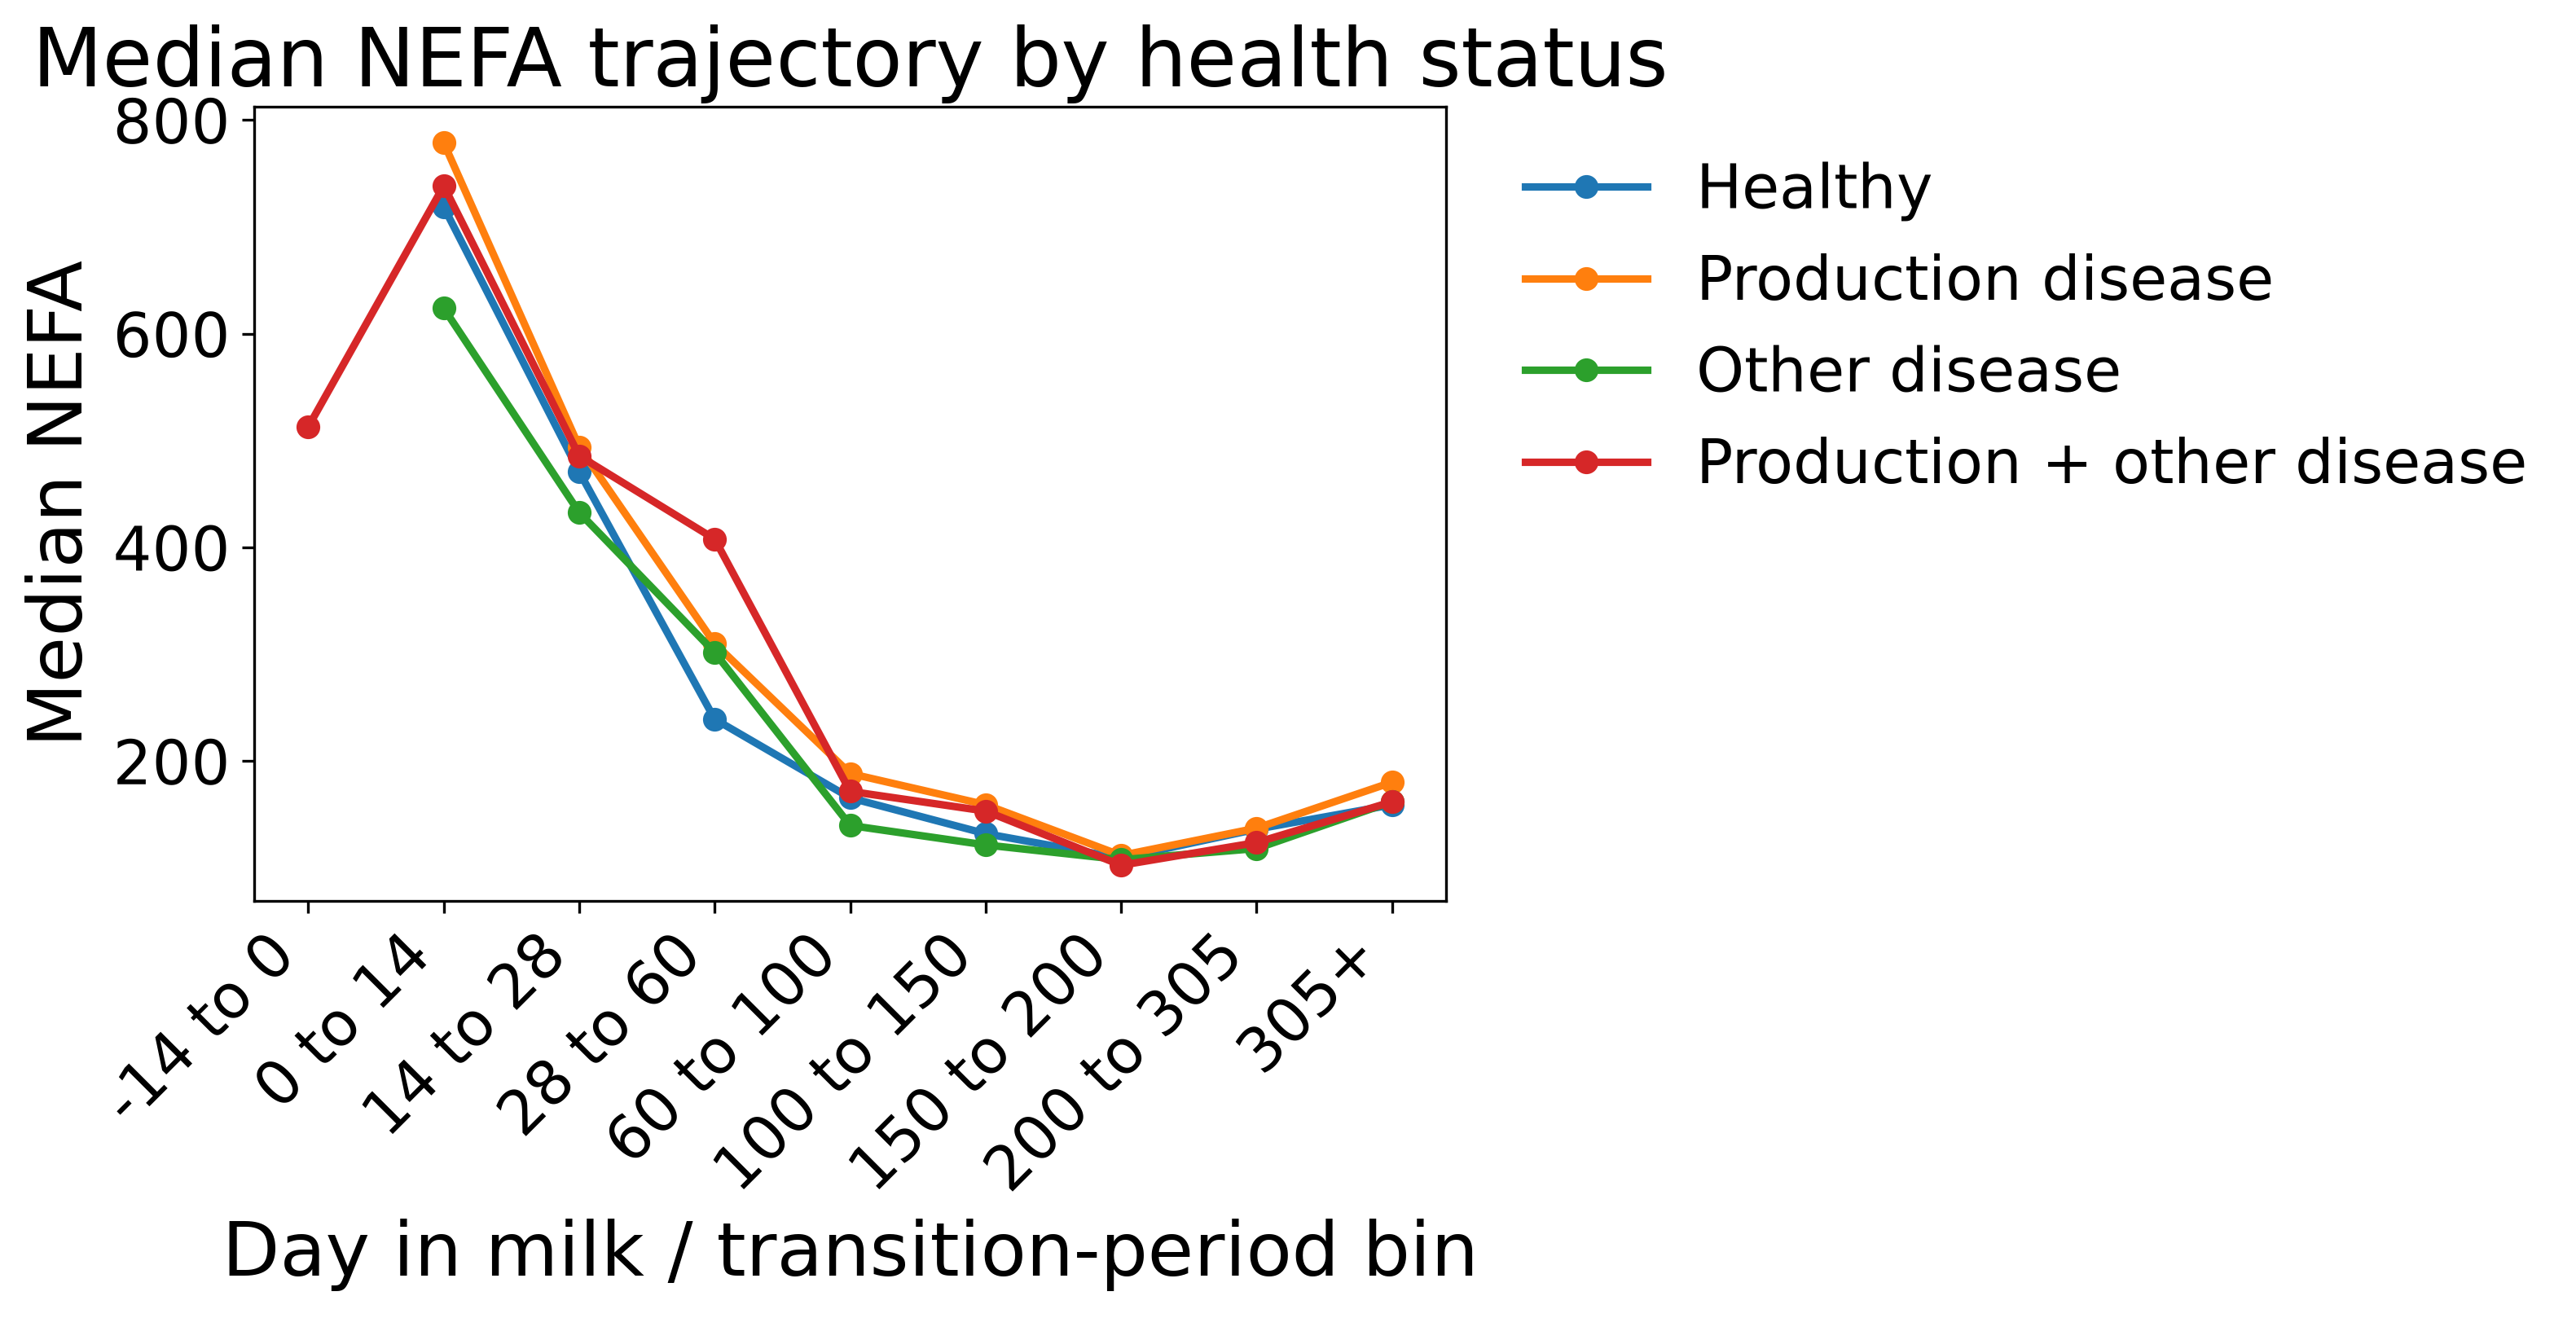
\includegraphics[width=0.95\linewidth]{../outputs/eda/figures/fig25_nefa_dim_trend_by_health_status.png}
\end{center}
\end{columns}

\end{frame}
%==================== SLIDE 14 ====================
\begin{frame}{Agenda for next week}

\setbeamercolor{item}{fg=tugreen}
\begin{itemize}
    \item Define the final analysis unit:
    \begin{itemize}
        \item daily record vs. lactation episode
    \end{itemize}
    \item Define the production-disease target clearly
    \item Decide the time window around calving
    \item Build preprocessing steps for sparse variables
    \item Prepare the first baseline modelling dataset
\end{itemize}

\end{frame}